\documentclass[a4paper]{article}
\textwidth = 450pt
\headsep = 2pt
\headheight = 1pt
\oddsidemargin = 1pt

\usepackage{changepage}
\usepackage{fancyvrb}
\usepackage{graphicx}
\usepackage{amsmath}
\usepackage{capt-of}
\usepackage{amsfonts}
\usepackage{verbatim}
\usepackage{courier}
\usepackage{float}
\restylefloat{table}

%%%%%%%%%%%%%%%%%%% Code %%%%%%%%%%%%%%%%%%%%%%
\usepackage{color}
\usepackage[table]{xcolor} %adding background color to your tables
\usepackage{listings}% Allows you to present C++ syntax as it looks
\usepackage{listings} %enables inputing code set the settings below
\definecolor{dkgreen}{rgb}{0,0.45,0}
\definecolor{gray}{rgb}{0.2,0.5,0.5}
\definecolor{mauve}{rgb}{0.58,0,0.82}
%\definecolor{purple}{RGB}}{204, 45, 109}
\lstset{ %
language=C, % choose the language of the code
commentstyle=\color{dkgreen},
basicstyle=\footnotesize, % the size of the fonts that are used for the code
numbers=left, % where to put the line-numbers
numberstyle=\footnotesize, % the size of the fonts that are used for the line-numbers
stepnumber=1, % the step between two line-numbers. If it is 1 each line will be numbered
numbersep=5pt, % how far the line-numbers are from the code
backgroundcolor=\color{white}, % choose the background color. You must add \usepackage{color}
showspaces=false, % show spaces adding particular underscores
showstringspaces=false, % underline spaces within strings
showtabs=false, % show tabs within strings adding particular underscores
frame=single, % adds a frame around the code
tabsize=2, % sets default tabsize to 2 spaces
captionpos=b, % sets the caption-position to bottom
breaklines=true, % sets automatic line breaking
breakatwhitespace=false, % sets if automatic breaks should only happen at whitespace
keywordstyle=\color{purple}, % keyword style
numberstyle=\tiny\color{gray}, % the style that is used for the line-numbers
rulecolor=\color{black}, % if not set, the frame-color may be changed on
stringstyle=\color{blue}, % string literal style
escapeinside={\%*}{*)} % if you want to add a comment within your code
}
\DefineVerbatimEnvironment{code}{Verbatim}{fontsize=\small}
\DefineVerbatimEnvironment{example}{Verbatim}{fontsize=\small}
%%%%%%%%%%%%%%%%%%%%%%%%%%%%%%%%%%%%%%%%%%%%%%%%

\begin{document}
\title{Using Kinect to Evaluate Dance Performances\\ Third Year Group Project}
\author{Stylianos Venieris, Marcin Baginski, Theo Pavlakou, \\Zeping Xue, Yijie Ge \& Hesam Ipakchi  }
\date{\today}
\maketitle
\pagenumbering{gobble}
\newpage

\pagenumbering{arabic}
\setcounter{page}{1}
\section*{\center Abstract}
\textbf{Not Done}

\section{Kinect \& NiTE Software Evaluation}
\noindent
To determine a method of evaluating the dance student, the limitations of the camera and the NiTE software must first be evaluated with respect to the criteria addressed below. To do this we use the UserViewer Application that comes as a sample with the NiTE software library with the camera elevated 75 cm above the ground, within the 60 cm to 180 cm range that is suggested by Microsoft for optimal tracking. 

\subsection{Camera Range}
\noindent 
To test for the camera's range, we lay a tape measure on the ground starting from directly below the camera up to 8 m away from the camera. We then use two subjects of different heights and body shapes to evaluate the performance of the camera and the software for tracking at different distances. The subject first starts within a few centimetres of the camera and slowly moves backwards until the camera calibrates and starts tracking and continues to do so until the tracking is lost. After this, the subject is required to start from the depths of the room, much further than the range of the camera, and to start walking slowly towards the camera, again taking a record of the following specifications. The results can be shown in Tables \ref{cam_range_180_away} to \ref{cam_range_150_toward}.
\\
\begin{table}[h]
\center
\begin{tabular}{ | l | c |}
\hline
Distance from Camera/cm & Description of Performance \\
\hline
60 & Identification of subject. Tracking. No skeleton.\\
120 & Skeleton fitted\\
410 & Tracking is lost\\
\hline
\end{tabular}
\caption{Subject moving away from camera. Subject height 180 cm.}
\label{cam_range_180_away}
\end{table}

\begin{table}[h]
\center
\begin{tabular}{ | l | c |}
\hline
Distance from Camera/cm & Description of Performance \\
\hline
100 & Identification of subject. Tracking. No skeleton.\\
120 & Skeleton fitted\\
410 & Tracking is lost\\
\hline
\end{tabular}
\caption{Subject moving towards camera. Subject height 180 cm.}
\label{cam_range_180_toward}
\end{table}

\begin{table}[h]
\center
\begin{tabular}{ | l | c |}
\hline
Distance from Camera/cm & Description of Performance \\
\hline
70 & Identification of subject. Tracking. No skeleton.\\
110 & Skeleton fitted\\
430 & Tracking is lost\\
\hline
\end{tabular}
\caption{Subject moving away camera. Subject height 150 cm.}
\label{cam_range_150_away}
\end{table}

\begin{table}[h]
\center
\begin{tabular}{ | l | c |}
\hline
Distance from Camera/cm & Description of Performance \\
\hline
50 & Identification of subject. Tracking. No skeleton.\\
110 & Skeleton fitted\\
430 & Tracking is lost\\
\hline
\end{tabular}
\caption{Subject moving towards camera. Subject height 150cm.}
\label{cam_range_150_toward}
\end{table}
\noindent
These results highlight the fact that the camera has a restricted field of view and therefore the number of people that each camera can support is limited. This will have to be further considered when finalising a design for the application. One thing to note is that, since  the optimum distance away from the camera, with respect to tracking, is in the range of 1.5m to 3.5m it would not be beneficial to have the camera(s) in the corners of the room. This would cause a huge amount of the already small range to be wasted due to the height of the room. 

\subsection{Effect of Varying Lighting Conditions}
\noindent
In order to evaulate the effect of varying lighting conditions on the tracking capabilities of the camera, we utilise a lux meter to determine the intensity of light in a room. The meter has been calibrated such that a complete darkness represents 0 lux. We then perform a series of tests to determine, if the varying lighting conditions have an effect on the tracking range of the camera. The table below presents the results of the tests:
\begin{table}[h]
\center
\begin{tabular}{ | l | c |}
\hline
Light intensity & Tracking range (starts - stops tracking) \\
\hline
4 lux & 120 cm - 420 cm\\
16 lux & 120 cm - 420 cm\\
44 lux & 120 cm - 420 cm\\
142 lux & 120 cm - 420 cm\\
176 lux & 120 cm - 420 cm\\
\hline
\end{tabular}
\caption{Tracking range in varying light intensity of the room}
\label{cam_range_varying_light}
\end{table}

\noindent
Since the skeleton is primarily fitted using the depth sensor of the RGB-D camera, the light intensity was expected to have little, if any, effect on the tracking range of the camera. Initially, we were expecting that the higher intensity of light might have a negative impact on the effectiveness of the IR depth sensor, however this has not been the case. It has been confirmed that varying light intensity, within bounds that we were able to achieve, have no effect on the range of the camera and its tracking capabilities.

\subsection{Obstruction in Range}
\noindent
To test for the possibility that obstructions could interfere with the fitting of the skeleton on the subject, we place a chair in various positions around the subject and in front of the subject. We then do the same with another person walking in the vicinity of the subject. This scenario is probably more relevant to the situations which may be encountered in a dance class room.  
\subsubsection{Chair}
\noindent Positioning the chair adjacent to the subject produces interesting results. When the subject is holding the chair, the NiTE software falsely identifies the chair as an extension of the subject's body and, thus, tries to fit a skeleton to the chair as well as the person. This can be seen in Figure \ref{lifting_chair}.

\begin{figure}[H]
\center
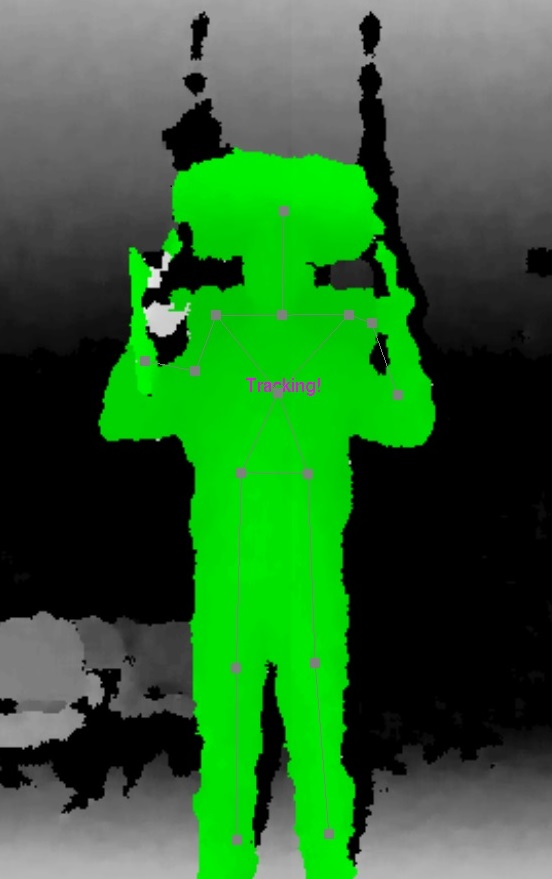
\includegraphics[scale=0.2]{Head_Chair.jpg} 
\caption{Subject is lifting the chair. NiTE cannot distinguish between the chair and the subject.}
\label{lifting_chair}
\end{figure}

Putting the chair directly in front of the subject at the level of its waits does not give the same result, but instead the proportion of the skeleton that is created by the software is quite distorted due to the reflection of the IR on the chair which does not allow the precise localisation and detection of the subject's obstructed parts. As Figure \ref{chair} illustrates the perceived angle of the subject's right leg appears to have a deviation angle of $45^o$ that does not agree with the actual leg position.

\begin{figure}[H]
\center
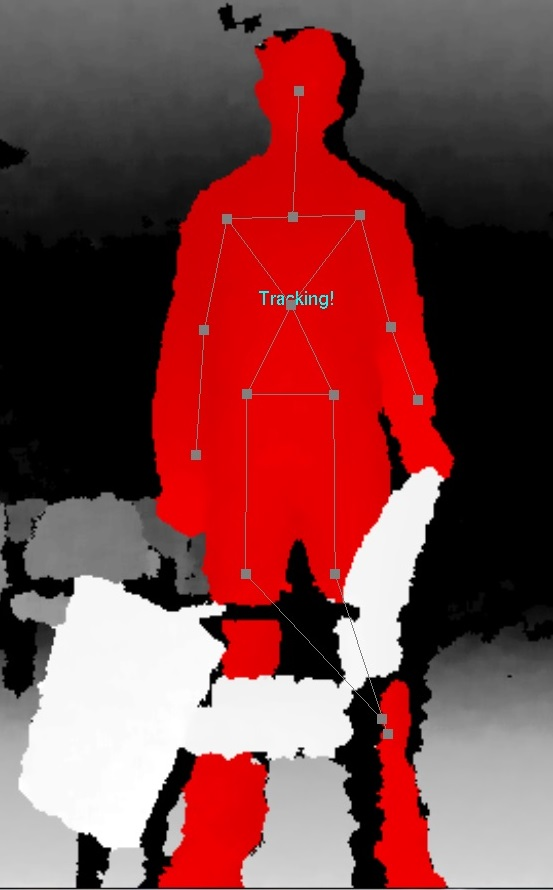
\includegraphics[scale=0.2]{Chair.jpg} 
\caption{Chair directly in front of the subject.}
\label{chair}
\end{figure} 
%% CHANGE
% Not finished. It seems that this section is quite a hand waving description of the experiment because we probably could have been more thorough.  
\subsubsection{Person}
\noindent
In this experiment, the second person walks within different ranges of the camera and the initial subject. Interestingly enough, even at quite fast speeds of movement, the camera can calibrate and track both people quite quickly. This will most probably not be a limitation when designing the software. Nevertheless, in the case where two dancers are dancing next to each other, the interference between their bodies distorts the received IR reading and the accuracy of the perceived joints' position deteriorates substantially.Figure \ref{occlusion1} indicates the inaccurate tracking of the right hand of one of the subjects due to its obstruction by the dancer on the left.

\begin{figure}[H]
\center
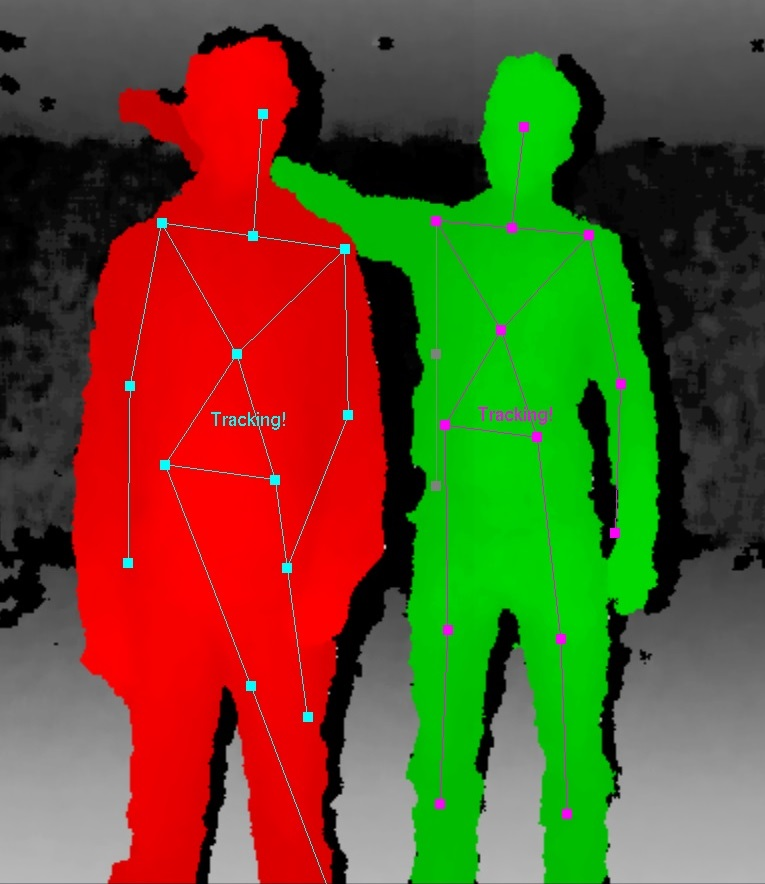
\includegraphics[scale=0.2]{Occlusion1.jpg} 
\caption{Adjacent dancers occlusion.}
\label{occlusion1}
\end{figure} 

Moreover, when a subject stands directly in front of another, NiTE is not always able to distinguish between the two subjects and thus it appears as if they are one body. This is shown in Figure \ref{occlusion3} below.

\begin{figure}[H]
\center
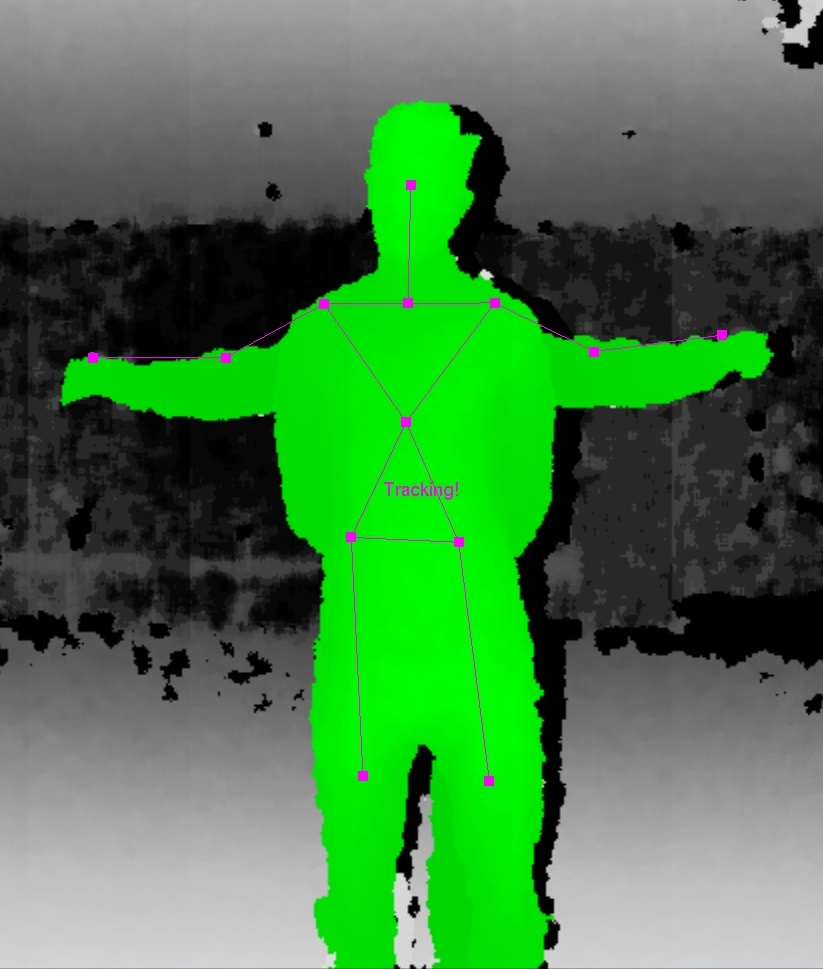
\includegraphics[scale=0.2]{Occlusion2.jpg} 
\caption{NiTE mistaking two skeletons for one.}
\label{occlusion3}
\end{figure} 

\subsection{Velocity of Movement}
Another important criterion regarding the performance of both the Kinect camera and the NiTE software package is the accuracy and responsiveness of the skeleton fitting. Our evaluation procedure consists of the recording of a predefined movement which would provide us with the subject's velocity information and would allow us to estimate how accurately the fitted skeleton is able to follow the actual move, by calculating the error between the perceived and the actual movement. In particular, we would record a slower and a faster versions of the same movement and compare the corresponding errors.

The subject's reference movement was determined to be a $180^o$ degrees right arm move starting from a vertical position with the hand facing the ceiling and following an arc. The testing procedure includes the modification of the \texttt{UserViewer} sample program in order to record twice the predefined movement as performed by the subject at high and low speeds. 

By capturing the recorded passage with a Desktop camera at a rate of 24 frames per second(fps), we are able to extract individual frames from the recorded videos. At this point, we define a starting and an ending point of the subject's right arm and select the frames that more accurately correspond to these positions. After following this procedure for both recordings, we end up with 3 frames from the fast and 16 from the slow version. The starting and ending position frames for the slow and the fast versions are shown below on Figure \ref{start_pos}. The substantial deviation between the shoulder-elbow vertex of the skeleton and the arm indicate the important increased error when the subject performs a fast move.

\begin{figure}[h]
\center
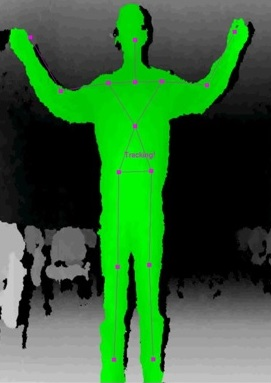
\includegraphics[scale=0.5]{SlowStart.jpg} 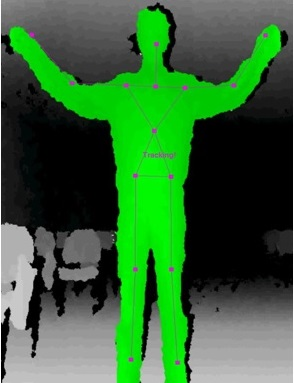
\includegraphics[scale=0.5]{FastStart.jpg}
\caption{Slow and fast recordings starting position.}
\label{start_pos}
\end{figure}

\begin{figure}
\center
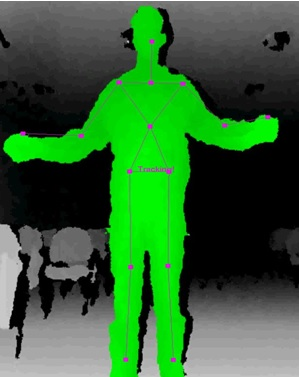
\includegraphics[scale=0.5]{SlowEnd.jpg} 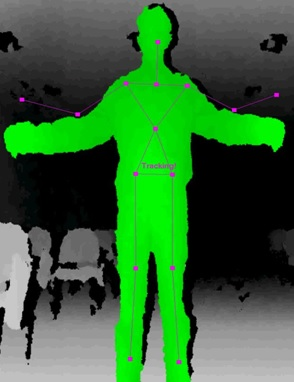
\includegraphics[scale=0.5]{FastEnd.jpg}
\caption{Slow and fast recordings ending position, with substantial error in the fast version's skeleton fitting.}
\end{figure}


\noindent A summary of the number of frames and the time between the starting and ending arm position for each  is shown below.

\begin{table}[H]
\center
\begin{tabular}{| c | r | r |}
\hline
Movement Speed & Number of Frames & Movement Duration/sec\\
\hline
Fast & 3 & 0.083\\
Slow & 16 & 0.670\\
\hline
\end{tabular}
\caption{Movement duration for fast and slow versions, recorded at 24 fps.}
\end{table}

The next step of the responsiveness evaluation is the estimation of the arm's actual starting and ending positions as well as its perceived position as defined by the fitted skeleton. As the arm follows an arc-shaped movement, we focus on measuring the angle between the subject's elbow and shoulder, with the shoulder  defined as the reference, and finding an estimate of the skeleton fitting error by comparing the actual angle and the angle of the vertex between the two joints with respect to the shoulder joint. Although both the actual and perceived starting positions are the same, the ending positions are different and result in errors in the subject's tracking. The angle measurements can be seen below in Table \ref{angle}.

\begin{table}[H]
\center
\begin{tabular}{| c | r | r | r |}
\hline
Movement Speed & Starting Angle/deg & Perceived Ending Angle/deg & Actual Ending Angle/deg\\
\hline
Fast & $3.5^o$ & $-30.5^o$ & $-55.3^o$\\
Slow & $4.4^o$ & $-49.2^o$ & $-64.0^o$\\
\hline
\end{tabular}
\caption{Perceived and actual starting and ending angles of the subject's arm.}
\label{angle}
\end{table}

The final step involved the estimation of the actual and perceived angular velocities based on the already obtained data and the calculation of the error as a consequence to the difference between them. By using the following formula, we estimate the angular velocities and the errors for both the slow and the fast recordings.
\begin{equation}
\omega = RotationalDisplacement * MovementDuration
\end{equation}

\noindent where \[RotationalDisplacement = EndingAngle - StartingAngle\]
and  $\omega$ stands for the angular velocity

\noindent The angular velocities and the corresponding errors for both the slow and the fast recordings are presented on the following table.

\begin{table}[H]
\center
\begin{tabular}{| c | r | r | r |}
\hline
Movement Speed & Perceived Angular Velocity/$^o/s$ & Actual Angular Velocity/$^o/s$ & Error/\% \\
\hline
Fast & $-408.0$ & $-705.0$ & $42.12\%$ \\
Slow & $-67.2$ & $-89.4$ & $24.8\%$ \\
\hline
\end{tabular}
\caption{Perceived and actual angular velocities and percentage errors.}
\end{table}



\subsection{Camera Angle Relative to Subject}
\noindent 
The fact that the application is to be used for the purpose of dancing means that an investigation into how the angle between the camera and the subject affects the results can help draw useful conclusions. For instance, in a certain dance the subject may turn so that only the profile is visible to the camera. Doing so without losing any information due to occlusion because of on of the arms or legs being covered by the rest of the body, may prove to be vital for the software to work effectively. 
\\\\
\noindent
To test for this, the subject stands in front of the camera, lifting both arms from the sides in the positive y direction up to $90^o$ and then back down. The subject then turns $90^o$ about the y-axis so that the right arm is in front of the camera, but the left arm is covered by the body. The results can be seen in Figure \ref{angle_camera}. As it can be seen here, at frame number 322 there is a peak in the y-coordinate of the right hand and the x-coordinate, but at frame 465 when the subject turns, only the y-coordinate changes. This is perfectly understandable since the the x-coordinate now stays roughly constant whilst the arm is raised. For the left arm however, both the x-coordinate and y-coordinate values are lost when the subject rotates, and thus there is a loss of information due to self occlusion. This may be a problem, however, as long as the teacher's information is also lost, it may not be.  
\begin{figure}[H]
\centering
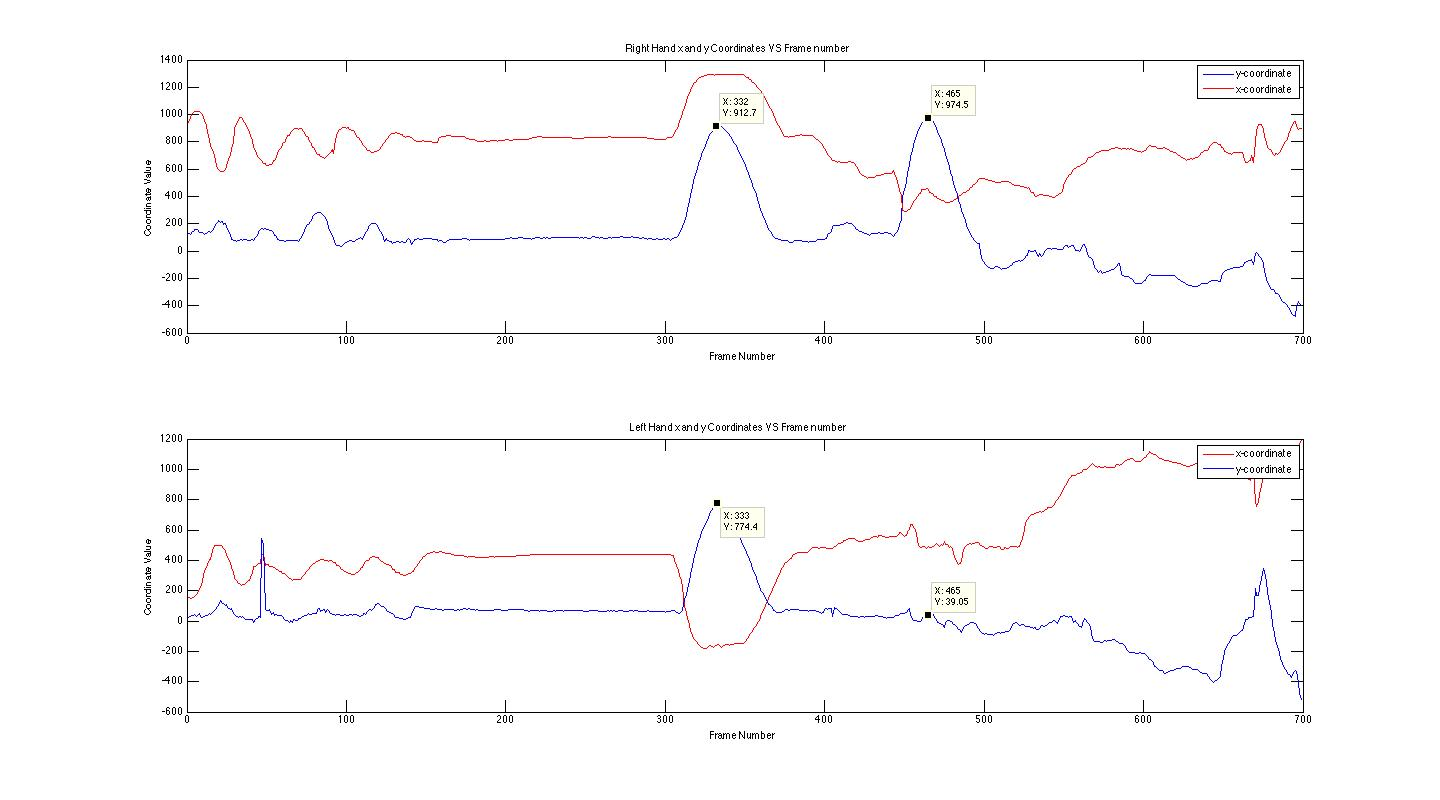
\includegraphics[scale=0.3]{Angle_To_Camera.jpg}
\caption{x and y coordinates plotted against frame number for the right hand and the left hand joints in experiment to see how angle to camera affects results.}
\label{angle_camera}
\end{figure}
 

\subsection{Multiple People}

\noindent
It may be necessary and efficient to use one camera to track multiple people and then process all the data in that way. This way fewer cameras would be needed for a particular class size with greater complexity being passed to the data analysis stages. \\\\
\noindent
In order to discover how many subject can be tracked by a single camera, we incrementally increase the number of people standing in front of the camera until the results are unsatisfactory for at least one of the skeletons. Unsatisfactory implies a skeleton deviating away from the body or discontinuity in tracking any of the joints. NiTE officially claims that the library can track as many people as can possibly fit physically in the camera range. We find that the maximum number of people that can fit in the cameras field of view with all joints showing 5. \\
 
\begin{figure}[H]
\centering
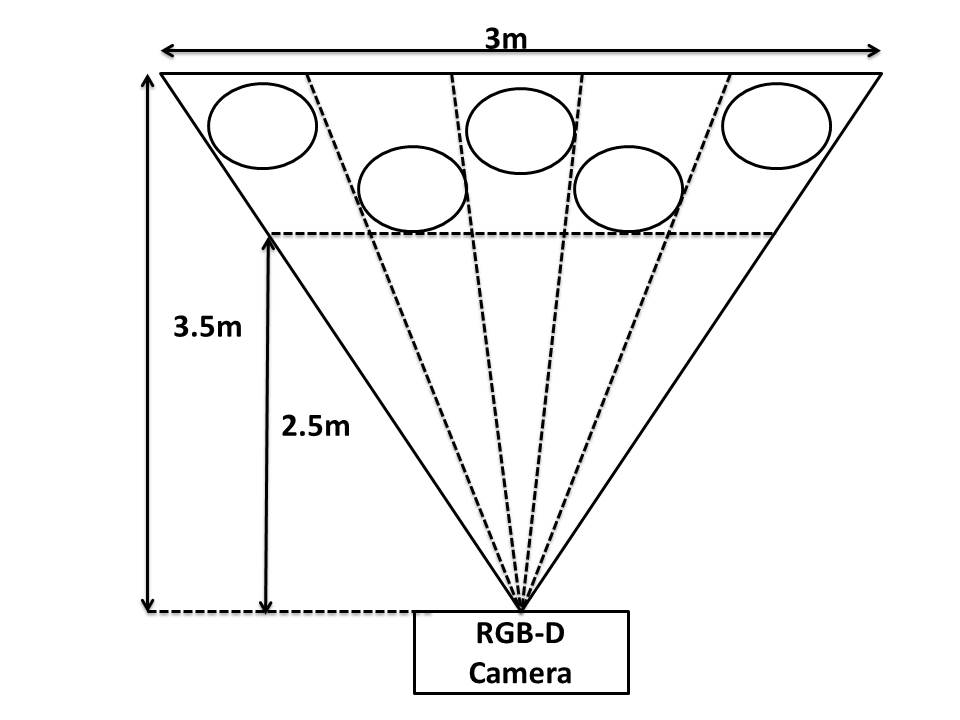
\includegraphics[scale=0.3]{multi_people1.jpg}
\caption{Position of five students with respect to the camera.}
\label{people_pos}
\end{figure}
 
\begin{figure}[H]
\centering
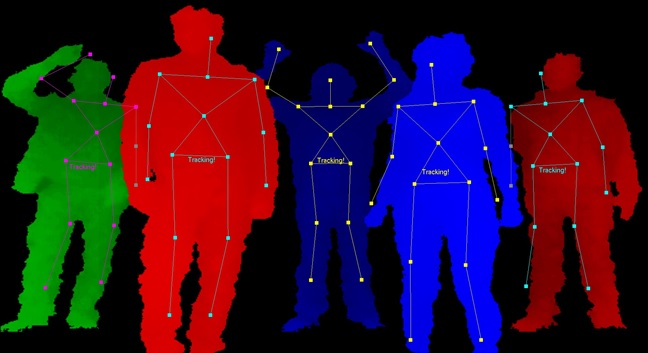
\includegraphics[scale=0.8]{multi_people2.jpg}
\caption{Five people being tracked in the configuration of Figure \ref{people_pos}.}
\end{figure}
\noindent
However, as mentioned before, a subject needs to be 2.5 to 4 metres away from the camera to be fully visible. Added to this, since the application of our software is for dancers, we need to provide an adequate spacing between students to allow for the movements involved in their practice. After splitting up the area for 5 subjects, each one has less than $1m^2$ of free space which is not considered enough for dancers. With 3 people for each camera however it will be able to provide a wide enough radius for each of the students.\\


\subsection{Multiple Cameras}
\noindent
Despite the various capabilities offered by a single Kinect camera, there are a number of weaknesses that can substantially limit the potential of its applications. Due to the active hacking community, the Kinect's specifications have been determined by reverse engineering the RGB camera, the IR laser projector and the 3-D depth sensor. An important result is that the angular field of view of the Kinect's RGB camera is limited to $62.7^o$ with the IR camera having a field of view of $57.8^o$. Given the aforementioned specifications and according to our testing, at an average working range of 2.5 meters, the depth image is only 3.5 meters wide. To overcome this obstacle and widen our field of view, additional Kinects can be used side by side. 

Another limitation which motivates the use of multiple Kinects is the fact that as the depth data sensed by the IR sensor come from a single direction, more accurate data is captured when the subject is perpendicular to the camera's normal. In particular, for our application whenever the subject stands with a profile view to the camera, data is lost and thus the subject's tracking would be less accurate. With multiple Kinects, a mixture of data from different angles can be captured and combined as necessary to increase accuracy and produce a more complete scene.

Nevertheless, the employment of multiple Kinects can lead to new obstacles. Research has suggested that using more than one camera with an overlapping region between them can lead to depth images that contain blind spots. To test whether this would be a problem in our application, we use the following initial setup.

\begin{figure}[H]
\centering
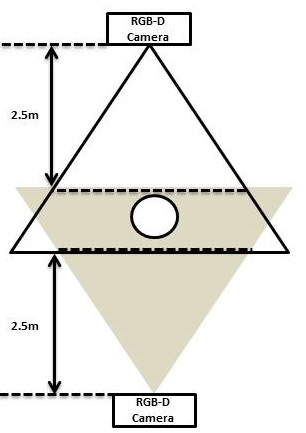
\includegraphics[scale=0.4]{figure_2cameras_opposite.jpg}
\caption{Initial configuration of two Kinects placed on opposite sides.}
\label{2_cameras_config1}
\end{figure}

We first record the camera's reading without a subject in the scene. As Figure \ref{IR_interference}. below shows, the IR interference caused by the Kinect on the opposite side of the room creates a substantial blind spot which confuses the algorithm that determines the depth and no useful depth data is captured.

\begin{figure}[H]
\centering
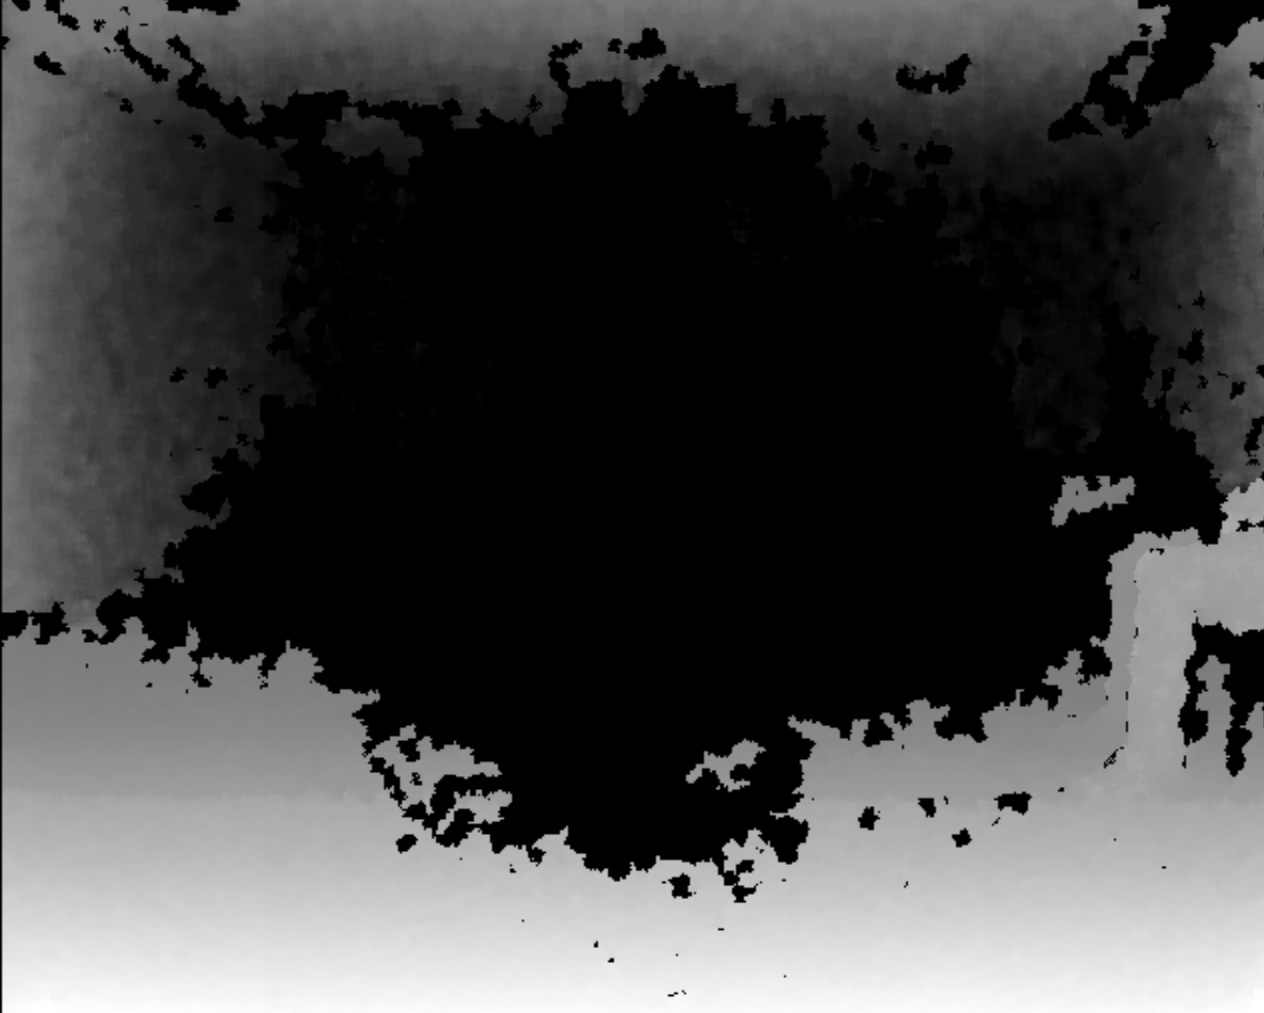
\includegraphics[scale=0.2]{IR_Interference2.jpg}
\caption{Interference between Kinects placed on opposite sides of the room.}
\label{IR_interference}
\end{figure}

When a subject comes in the scene, although it is tracked, the interference still poses a problem by distorting the left hand of the subject as shown in Figure \ref{IR_interference_w_subject}. Such a distortion is intolerable to our application. 

\begin{figure}[H]
\centering
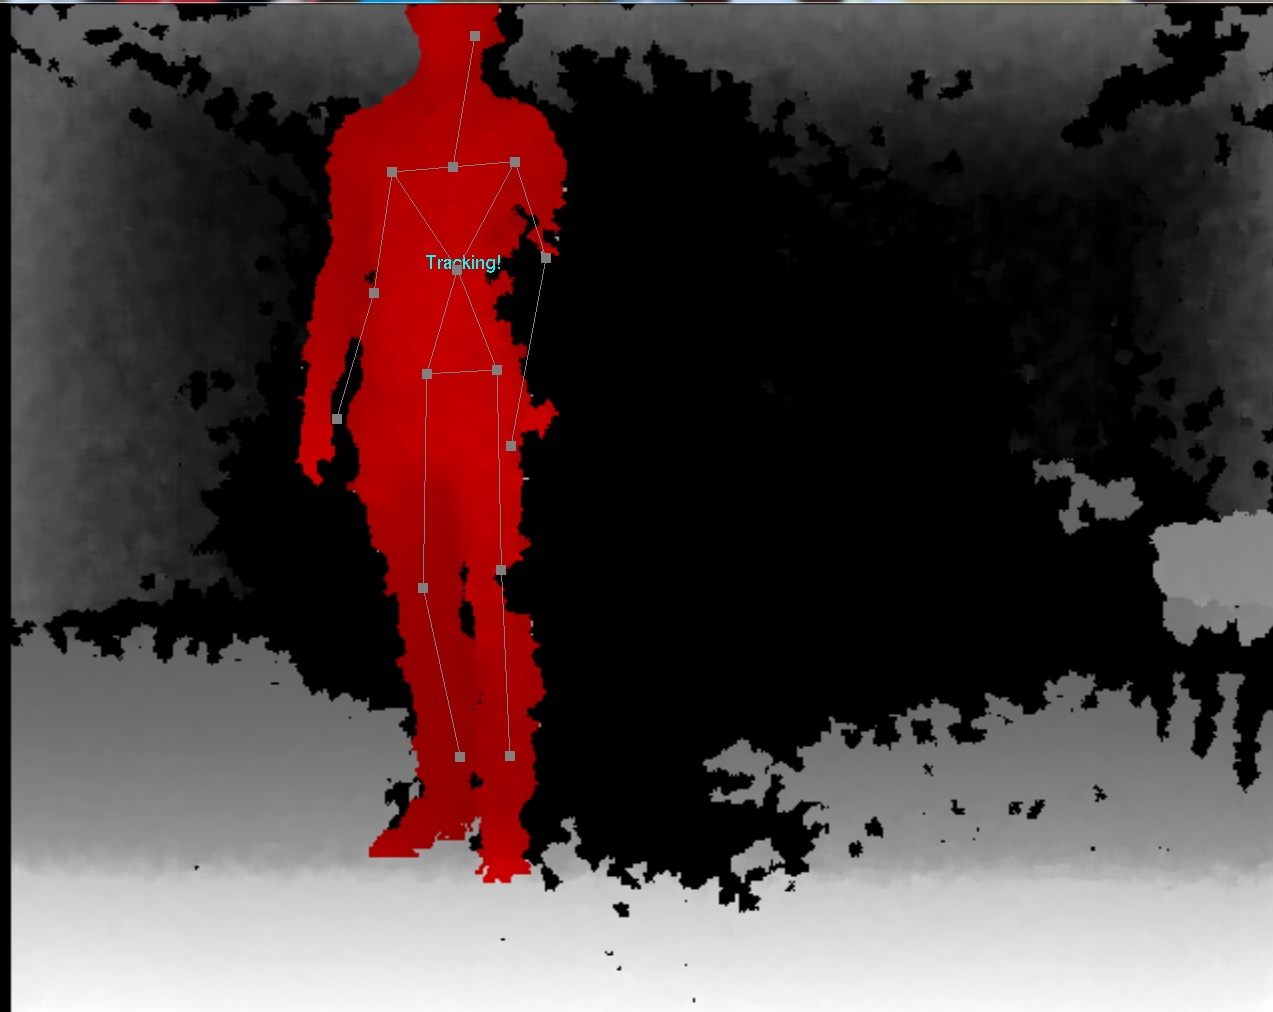
\includegraphics[scale=0.2]{IR_Interference3.jpg}
\caption{Interference between Kinects placed on opposite sides of the room with subject.}
\label{IR_interference_w_subject}
\end{figure}

A more useful configuration includes the placement of the second Kinect in such a way that the IR illumination patterns of the two cameras create an angle of $90^o$ so that any joints not visible to one camera, may be visible to the other. This also means that their field of view overlap is minimised. Such a configuration can be seen below in Figure \ref{2_cameras_config2}.

\begin{figure}[H]
\centering
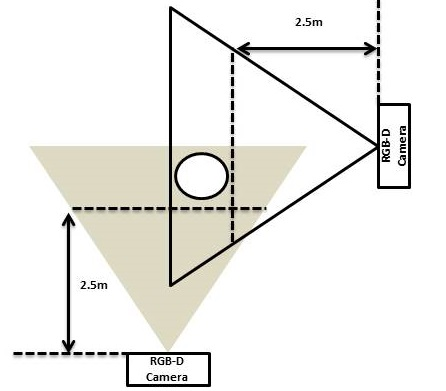
\includegraphics[scale=0.4]{figure_2cameras.jpg}
\caption{Configuration of two Kinects in order to minimise overlap.}
\label{2_cameras_config2}
\end{figure}

In this case, a recording of the camera's view without a subject gives us a much lower level of interference compared to the initial configuration. This can be seen in Figure \ref{IR_interference_90}.

\begin{figure}[H]
\centering
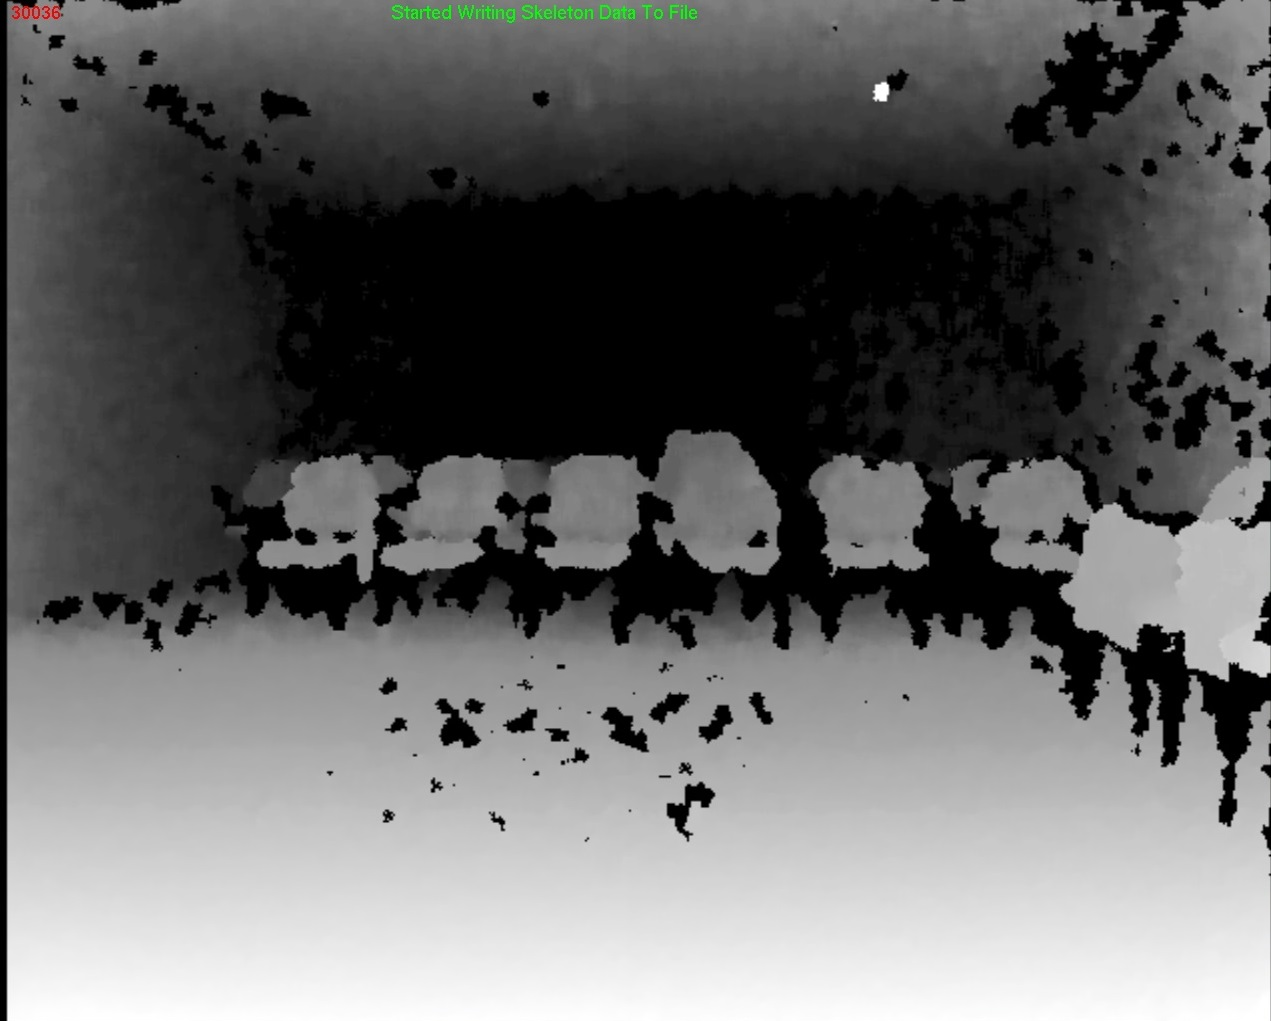
\includegraphics[scale=0.2]{IR_Interference90deg.jpg}
\caption{Interference between Kinects placed in a $90^o$ angle.}
\label{IR_interference_90}
\end{figure}
 
In our experiment, the subject is asked to stand still in front of the camera with arms to the side for about 5 seconds. This is initially done four times with a single camera. The measured data is used as a reference when comparing to a two-cameras configuration. The same measurements are taken for two cameras placed in a $90^o$ angle. In this way, the effect of the interference can be quantified by comparing the two set of data. The method we follow to compare the sets of data is by comparing the mean of the standard deviations for each trial. This is illustrated in Figure \ref{Multiple_Std}. 
 
\begin{figure}[H]
\centering
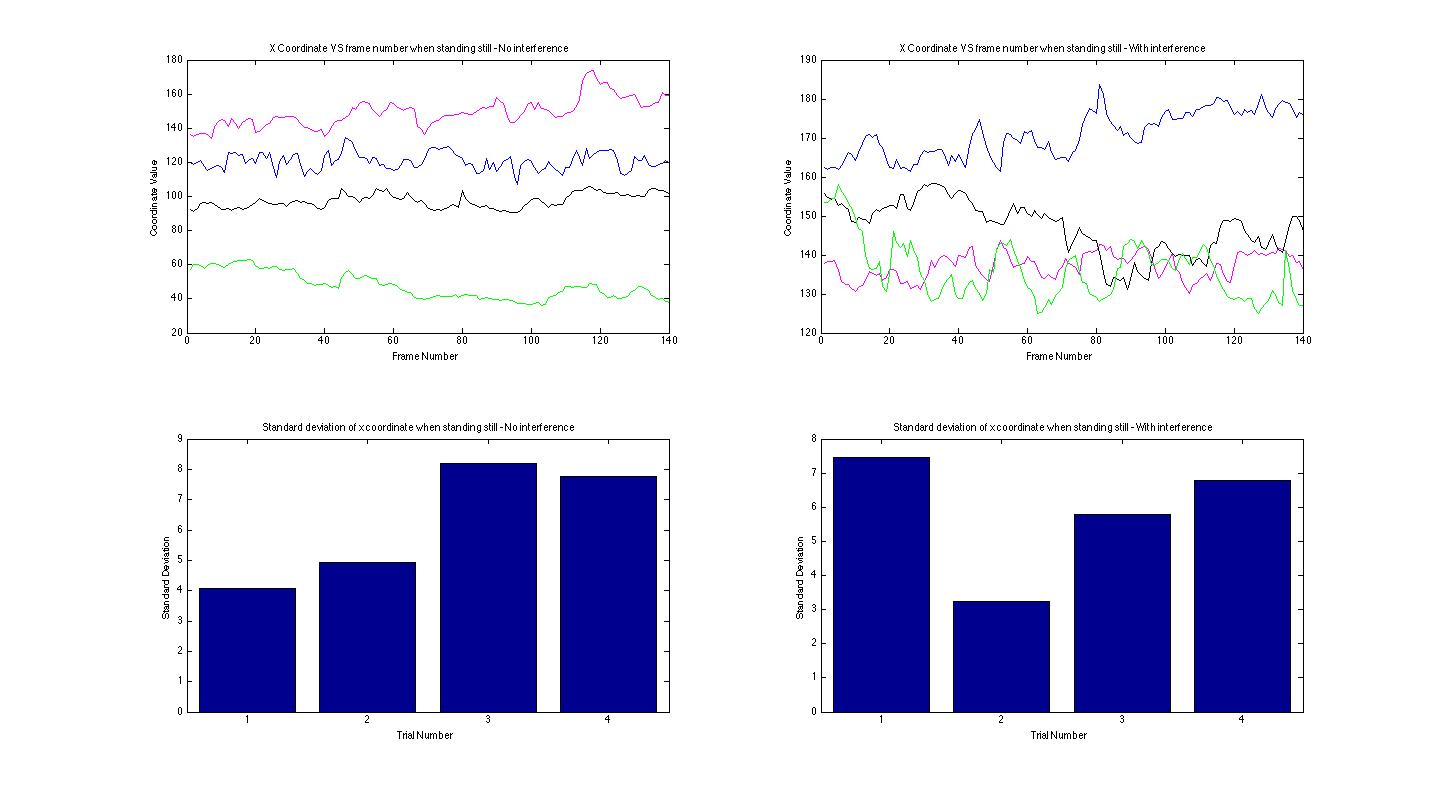
\includegraphics[scale=0.3]{Multiple_Cameras_Std.jpg}
\caption{Multiple Cameras Data.} % CHANGE
\label{Multiple_Std}
\end{figure}

As it can be seen above, both sets of data give very similar standard deviations and consequently the mean standard deviation with no interference, $\sigma_{ni}$, is 6.2412 units whereas when interference is present $\sigma_{i}$ is 5.8198 units. As the numbers indicate, both have roughly equal magnitude and given the small sample size, they can be considered equal. Moreover, as the dynamic range of an average signal is in the range of 400 to 800 units, the difference between the means is insignificantly small and, as a result, the interference introduced in this configuration is tolerable for the purpose of our application.

\subsection{Analysis of Results}
\noindent
During our preliminary tests, the camera range which allows subject tracking and skeleton fitting was determined to be within 1.2 - 4.1 metres. While it is more than enough for various video game applications, the range would clearly be a significant constraint when trying to implement the camera tracking in a dance studio. From this result we can immediately rule out the idea of placing multiple cameras in elevated positions of a room, since such positioning would further reduce the already small tracking range.

\medskip \noindent While the lighting conditions of a room had absolutely no effect on the tracking capabilities of the camera, we determined that various objects in the vicinity to the subject can sometimes be wrongly identified as parts of the body. Additionally, the ones further away from the tracked person might disrupt the continuity of the skeleton tracking and the data reported from it. We determined, that the nubmer of people who can be actively tracked with the NiTE software is not restricted in any way other than how many can physically fit in the range of the camera, however any occlusion between them and the camera can create a serious challenge in assessing the performance of multiple dance students. In other words, it might be difficult to automatically assess the performance of multiple dancers in front of the same camera, due to the nature of this activity, during which the performers will inevitably obstruct themselves.

\medskip \noindent We also determined that there is a significant correlation between the dancer's speed of movement and the error in the skeleton's data with respect to the actual position of the subject. During very fast moves, the skeleton sometimes lags significantly behind the subject, which may lead to losing some data precision. This will however depend strongly on the nature of the dance move and its effect on the assessment of the student is unclear at this point.

\medskip \noindent As mentioned in the previous sections, some dance moves may require the performer to turn around and therefore cover some parts of their body from the camera. This unwanted, yet also unavoidable issue can partially be resolved by placing multiple RGB-D devices close to each side of the subject. This however poses another problem of the interference between them. We will investigate the actual cost/performance ratio of this solution in the following sections, when we will evaluate the performance of the automatic scoring algorithms with respect to the data from multiple cameras.

\clearpage

\section{Automatic Evaluation of Students}
\noindent
This section discusses the way in which the application will be used to evaluate the student's performance with respect to the teacher's. The software will have to detect errors that the student has made, detect time periods in which the student performed poorly as well as satisfactory and be able to give a few other useful statistics for the teacher to also grade the student. Using only information from the data points of the joints from NiTE and the RGB-D stream from OpenNI, various things need to be considered and multiple modules will need to be created to handle the data. 

\begin{figure}[H]
\centering
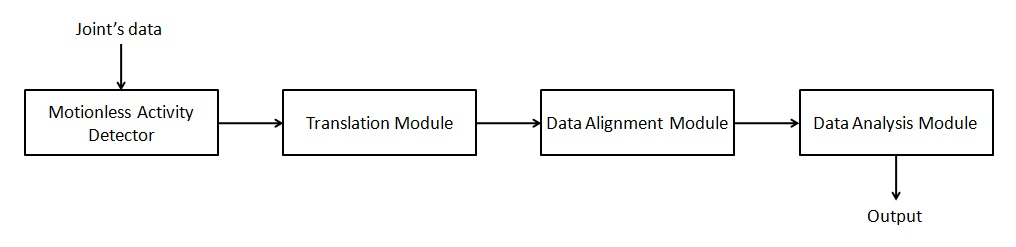
\includegraphics[scale=0.4]{data_analysis_modules.jpg}
\caption{High level design of modules necessary for automatic evaluation of student data.}
\label{modules}
\end{figure}
 
\noindent The design will consist of various modules, as seen in Figure \ref{modules}, that will divide the tasks into manageable chunks, which will be very helpful when trying to develop the software due to the level of abstraction associated with each piece of data. The algorithms will first be developed in Matlab, due to ease of use making the development of the algorithms as fast as possible, and then will be ported to C++, due to its speed and ease of integration with the development environment being used to develop the rest of the software. 

\subsection{Motionless Activity Detector}
\noindent 
With the current design in mind the student will be asked to first move slightly so that the NiTE software can calibrate and start tracking. After this, the student will be required to stand still in a predefined position for a minimum amount of time, to be decided later, afterwhich the student may start dancing. This will be the position that the next module will use to translate the coordinates with respect to a specific origin. The purpose of this module is to find a frame number during which the student will be in the standing still phase.\\\\
\noindent 
The algorithm is simple. Under the assumption that there is a time period in which there is relatively little movement the algorithm is only required to find a period with the least sum of the absolute change in all the coordinates. The aforementioned ``period'' takes the form of a non-overlapping sliding window over the joint data, for each joint. This sliding window has to contain the data of less than half the number of frames that are recorded in the minimum time period of motionless activity so that a frame within that period of time can be found, if the student did indeed stand still for the period of time. The window must be sufficiently large however to get a sum over a wide enough range of values so that momentarily motionless activity is not detected instead at some other point.\\\\
\noindent
The initial algorithm is of the form:
\begin{itemize}
\setlength{\itemsep}{1pt}
\setlength{\parskip}{0pt}
\setlength{\parsep}{0pt}
	\item Make a sliding window of 10 to 14 frames.
	\item Take the sum of the absolute difference between the frames for each of the coordinates (x, y, z).
	\item Find the window with the minimum for the sum of absolute derivative of the positions of the coordinates between frames.
	\item Get initial index of that frame.
\item Do this for all major joints and make sure all initial indices match.
\item If they do not all match, take the majority. 
\end{itemize}
\noindent
To test this we perfom various tests.
\subsubsection{Test for One Joint}
The first step is to check that the algorithm works for only one joint, chosen to be the right hand. The subject moves the right hand until the \texttt{UserViewer} calibrates and starts tracking, then holds the hand in a certain position for a minimum of 1 second, and then moves it again. The data from all the points is then printed to a file, in a form that can be loaded by Matlab into a matrix and our algorithm is used to find the stationary point. \\\\
\noindent
To confirm our results, a plot of the graph for the coordinate's positions versus frames is created and the video is also watched with the frame number in the top left corner. If the frame number returned by the algorithm corresponds to a time period in which the subject is still, this is taken as a correct result. 
\subsubsection{Test for Multiple Points}
\noindent 
In this test the subject walks in front of the camera moving their limbs until tracking commences, then stands still for 1 second and then moves again. Variations of this are tested in which all body parts are used, the upper half and the lower half. Once again, the data is processed by the Matlab scripts created but this time a vector of results is returned by the algorithm. Each result in the vector is the stationary point for each joint for each of the coordinates (x, y, z). The algorithm then takes the frame value that has the highest occurrence in the vector and returns this as a frame in which there is no motion of the subject. The same criteria as in the previous test is used to measure the correctness of the algorithm. 

\subsubsection{Obstacles Encountered}
\noindent
Various problems have arisen during the tests. The first problem is associated with the data itself. The data comes in a 4-tuple for each joint, representing the (x, y, z) coordinates and the fourth value is the confidence level. This is a basic measure for how reliable the reading is of a particular point. When the confidence level is equal to zero, the coordinates of the previous data point is used. This presents a problem for our initial algorithm however, because it works with differences between frames, and so if the confidence value is equal to zero, which happens often enough, the difference is also zero even when there is alot of activity taking place. To counter this, we change the algorithm so that, if two adjacent data points have the same value, a very large difference is associated to them. The probability of having results that are exactly equal is significantly low as the number of significant digits in the data is quite high, and empirically this has proven to be the case.\\\\
\noindent
Another issue is concerned with the number of frames to use for the window size. A large window size means that a much more reliable conclusion from the results can be drawn, as the sample size increases, but at a cost that the student has to stand still for a longer period of time, since the window size time should be less than twice the time period of no motion. This means a good balance has to be found. On the one hand, making the student stand still for too long deteriorates the user experience. On the other hand, the smaller the window size, the more susceptible to detecting temporary motionless activity within the dancing period. From the experiments, it has been found that a frame size of 30 frames makes the best compromise and means that the student must stand still for at least two seconds. This is not a problem, however, since other commercial software for different purposes requires a stand still period which is of a similar magnitude, such as facial recognition systems in airports. \\\\
\noindent
A further complication is that the number of frames shown in the .oni file recording is greater than that of the data in the file processed by Matlab. This means that the offset has to be found by writing to a separate file the starting frame when the first piece of data is written to the frame processed by Matlab. 



\subsubsection{Results}

\begin{table}[H]
\center
\begin{tabular}{| c | r | r | r | r | r | r | r | r |}
\hline
Coordinate & L Elbow & R Elbow & L Hand & R Hand & L Knee & R Knee & L Foot & R Foot \\
\hline
x & 241 & 211 & 241 & 241 & 241 & 241 & 211 & 211\\
y & 211 & 211 & 211 & 241 & 181 & 181 & 181 & 151\\
z & 211 & 211 & 241 & 241 & 211 & 211 & 151 & 211\\
\hline
\end{tabular}
\caption{Frame returned for Test Case 1 - Moving all body parts. The frame number which is in the majority here is 211.}
\label{angle}
\end{table}

\begin{table}[H]
\center
\begin{tabular}{| c | r | r | r | r | r | r | r | r |}
\hline
Coordinate & L Elbow & R Elbow & L Hand & R Hand & L Knee & R Knee & L Foot & R Foot \\
\hline
x & 301 & 211 & 301 & 301 & 301 & 271 & 271 & 271\\
y & 301 & 271 &  31  & 271 & 271 & 301 &  31  &      1\\
z & 211 & 211 & 241 & 241 & 211 & 211 & 151 & 211\\
\hline
\end{tabular}
\caption{Frame returned for Test Case 2 - Moving only upper body parts. The frame number which is in the majority here is 301.}
\label{angle}
\end{table}

\begin{table}[H]
\center
\begin{tabular}{| c | r | r | r | r | r | r | r | r |}
\hline
Coordinate & L Elbow & R Elbow & L Hand & R Hand & L Knee & R Knee & L Foot & R Foot \\
\hline
x & 91 & 91 & 151 & 91 & 121 & 151 & 151 & 91\\
y & 91 & 91 & 121 & 91 & 91 & 151 & 151 & 61\\
z & 121 & 121 & 121 & 91 & 121 & 121 & 151 & 121\\
\hline
\end{tabular}
\caption{Frame returned for Test Case 3 - Moving only lower body parts. The frame number which is in the majority here is 91.}
\label{angle}
\end{table}

\noindent
Though there are quite a few different values returned, there are 2 or 3 ones that are in a significant majority in either case. These are usually only separated by a window or two at most which corresponds to the majority of the frames returned being in a period of three seconds from each other. Since the subject usually stands for about 3 to 4 seconds, in our specific scenario, these results are valid as confirmed below.
\begin{figure}[h]
\center
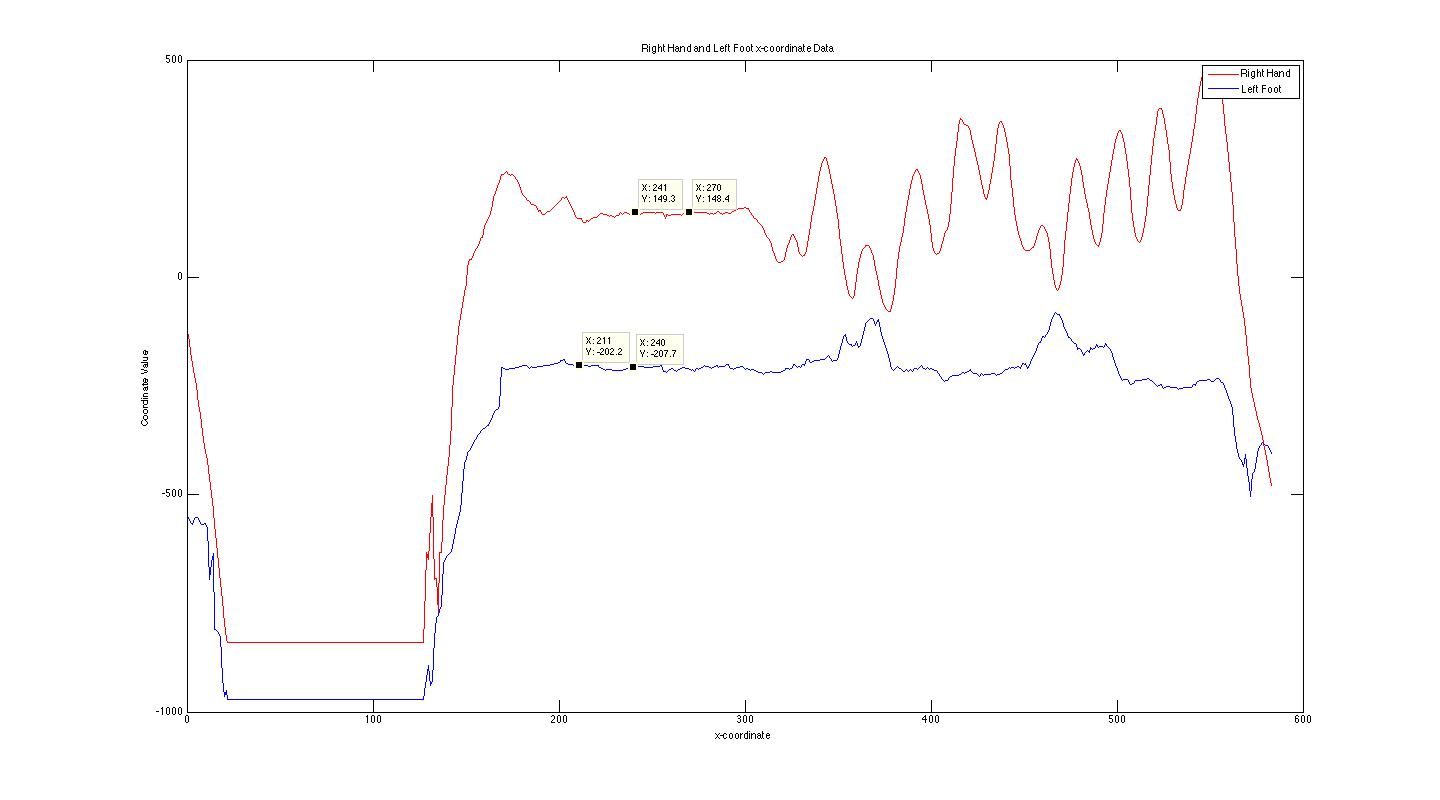
\includegraphics[scale=0.3]{Motionless_R_Hand_L_Foot_X.jpg} 
\caption{The x-coordinate data plotted for the right hand and the left foot of Test Case 1. The frames which are returned from the algorithm are shown on the graph.}
\label{motionless_rh_lf}
\end{figure}
\\\\
\noindent
As it can be seen from Figure \ref{motionless_rh_lf} though the frame numbers that are returned are different, both are in fact in a region of relatively little activity, and as confirmed by the video are within the period that the subject is standing still. 

\clearpage
\subsection{Translation Module}
\noindent
The purpose of the Translation Module is to take the original joint's positions data and remove the information which only adds unnecessary complexity, such as the exact position of the subject in the view of the camera. This is needed, because when we are comparing two dance moves, we do not want the score to be affected by the position of the dancers in the range of the camera e.g. in one recording the subject is standing on the left, in the other on the right. In order words, the score should be based only on what moves the dancers perform, not where do they perform them. In order to achieve that, we are going to shift all joint's positions so that they are relative to the torso joint, which we treat as the origin of the coordinate system.

\subsubsection{Algorithm Description}
\noindent
The initial algorithm is of the form:
\begin{itemize}
\setlength{\itemsep}{1pt}
\setlength{\parskip}{0pt}
\setlength{\parsep}{0pt}
	\item Find the number of the starting frame using Motionless Activity Detector.
	\item Crop the original data to begin from the starting frame.
	\item Find the (x, y, z) coordinates of the torso during the motionless activity by using the frame number obtained in the first step.
	\item For all joints: subtract the coordinates of the torso.
\end{itemize}

\subsubsection{Testing}
\noindent
In order to test the algorithm, we record two videos, where the subject performs the same movement in completely different parts of the camera range. Because of that, we are expecting the original data to be of similar shape, but have different absolute values. After running the algorithm on the data, the offset should disappear and the signals should be similar in both their shape as well as in absolute values.
\\
\begin{figure}[h]
\centering
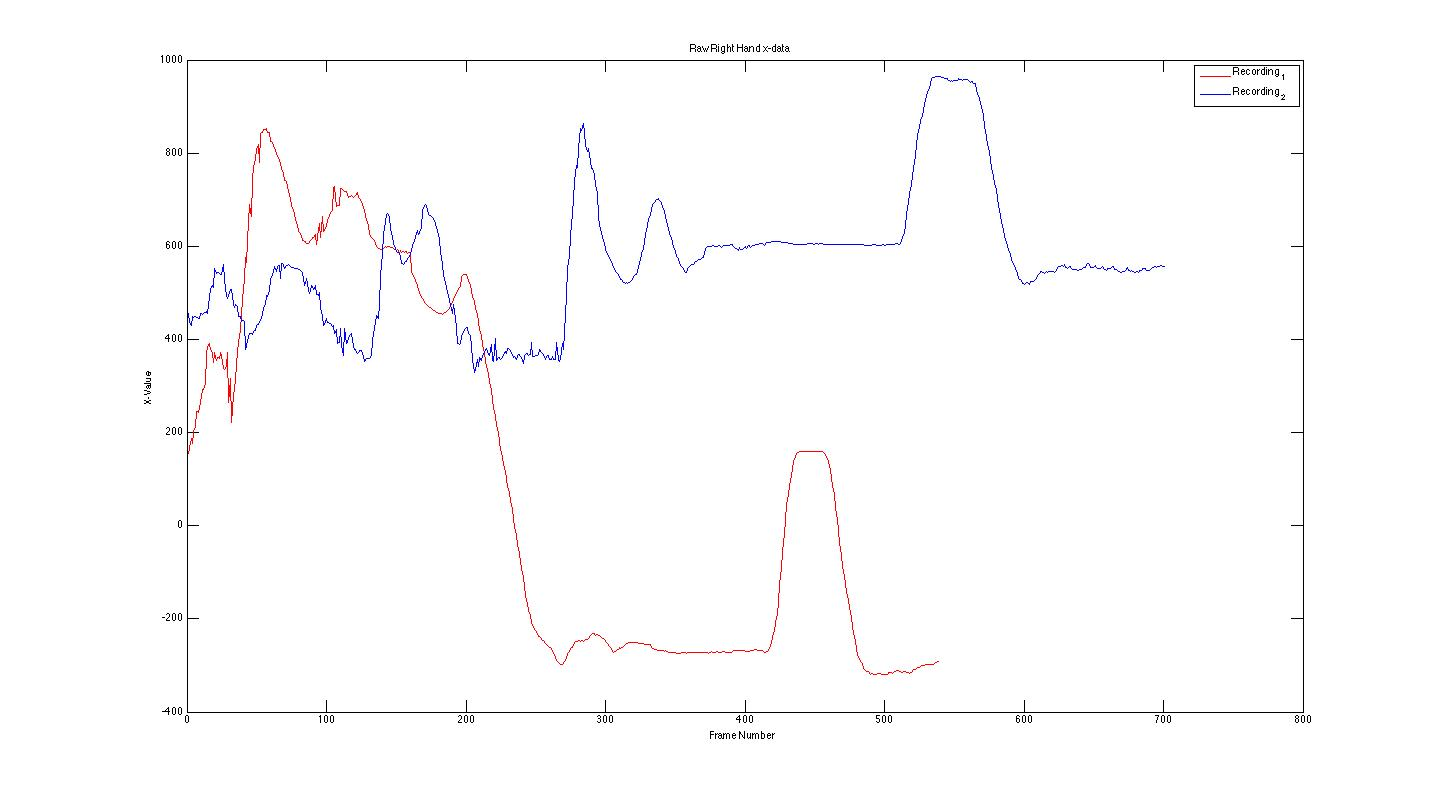
\includegraphics[scale=0.3]{Non_Translated_R_H_Data.jpg}
\caption{Right Hand data from two recordings before translation}
\label{pre_translation_graph}
\end{figure}

\begin{figure}[h]
\centering
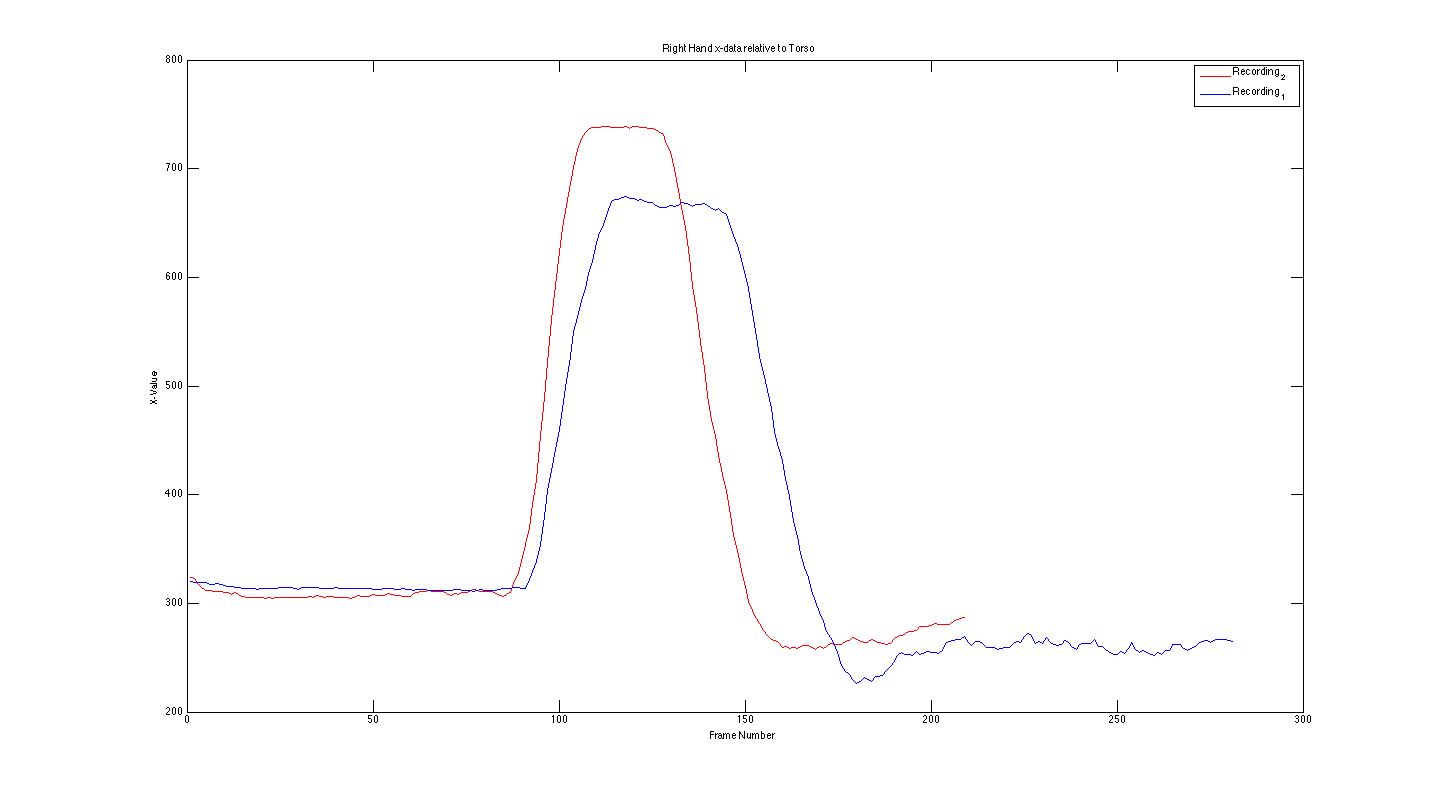
\includegraphics[scale=0.3]{R_H_Data_Relative_Torso.jpg}
\caption{Right Hand data from two recordings after translation}
\label{post_translation_graph}
\end{figure}

\noindent
Figure \ref{pre_translation_graph} shows the original data from two recordings for the right hand joint. Clearly, in both recordings, near the end the subject performs the same movement which is indicated by a spike in signal's value from being relatively constant. However, the absolute values of both signals do not correspond.
\\\\
\noindent
Figure \ref{post_translation_graph} shows the same signal after running it through the Translation Module. Now, the signal does not contain the initial calibration data any more. Additionally, both the shape and the absolute values of the signal are close to each other, which is the desired outcome.

\clearpage
\subsection{Scaling Module}
\subsection{Data Alignment Module}
\noindent
The purpose of the Data Alignment Module is to identify the frame shift between two similar dance moves and then align the signals, making it possible for them to be compared. The raw data will always be significantly misaligned, since it is virtually impossible for two people to start performing the dance at the exact same fraction of a second. The problem is visualised in figure \ref{pre_post_alginment} which shows the initial misalignment between two signals as well as the result of passing them through the Data Alignment Module.

\subsubsection{Algorithm Description}
\noindent
The first algorithm, which was eventually modified, was of the form:
\begin{itemize}
\setlength{\itemsep}{1pt}
\setlength{\parskip}{0pt}
\setlength{\parsep}{0pt}
	\item Calculate the cross-correlation between the teacher and student for every joint's x and y dimension.
	\item For every cross-correlation, identify the frame lag for which the cross-correlation has the biggest value.
	\item Calculate the mean of the frame lags and return it as the most likely misalignment value.
\end{itemize}
This version of the algotithm caused problems described in Section 2.4.3 and therefore the last step was changed to:
\begin{itemize}
\setlength{\itemsep}{1pt}
\setlength{\parskip}{0pt}
\setlength{\parsep}{0pt}
	\item Calculate the mean and standard deviation of all frame lags for which the cross-correlation has the highest value.
	\item Discard the frame lags which lie outside of one standard deviation of the mean.
	\item Calculate the average value of all other frame lags and return it as the most likely misalignment value.
\end{itemize}

\subsubsection{Testing \& Results}

\begin{figure}[h]
\centering
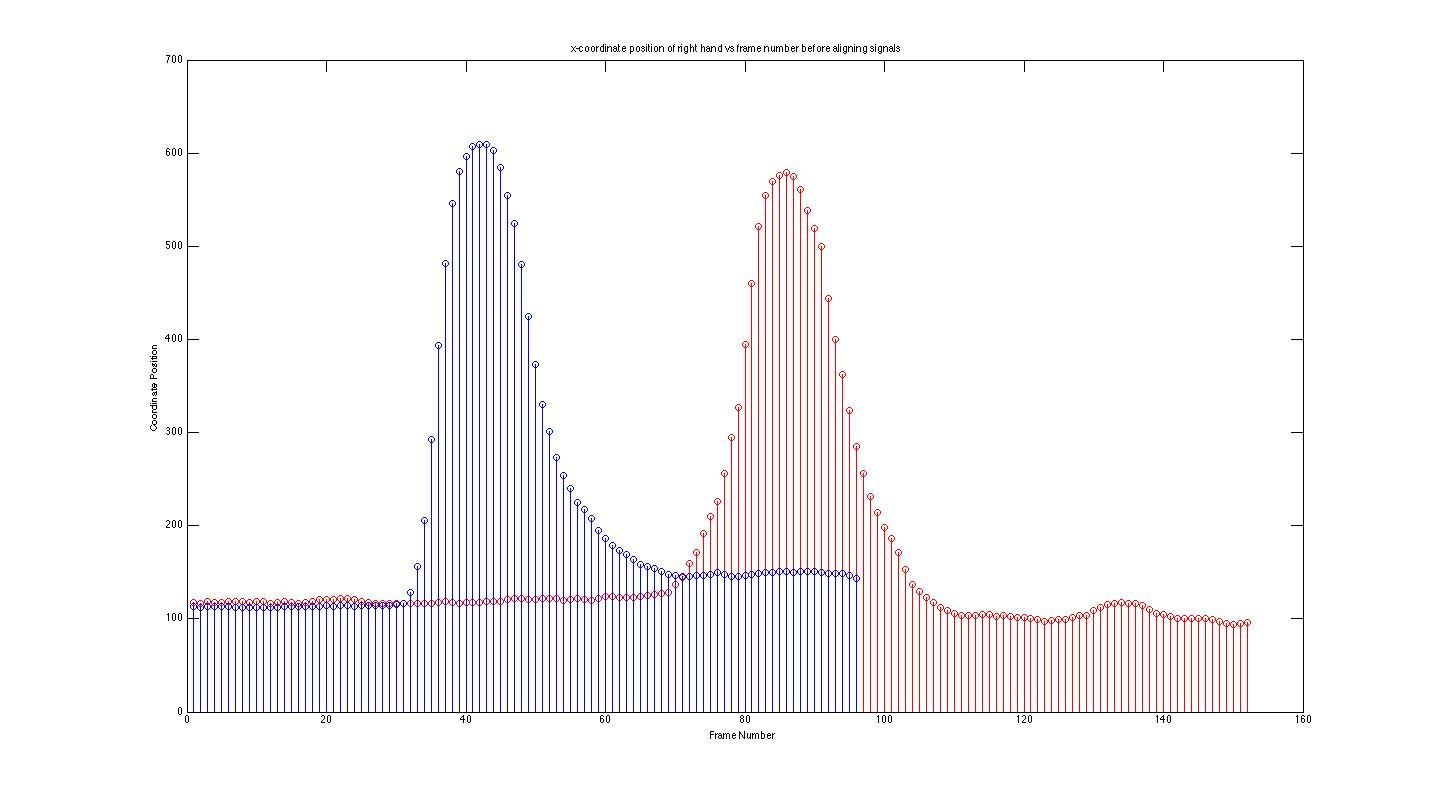
\includegraphics[scale=0.2]{Initial_Frame_Det_Before.jpg}
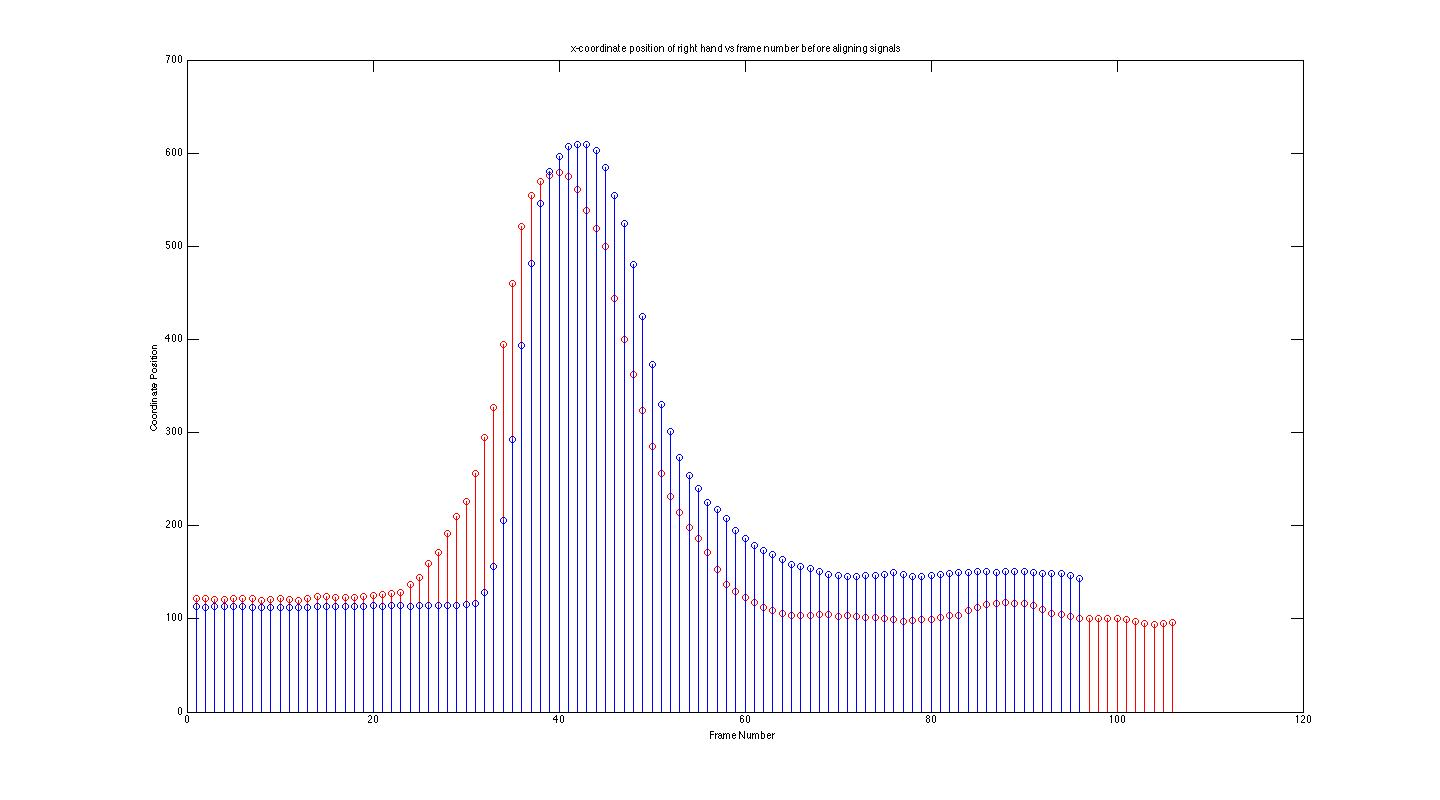
\includegraphics[scale=0.2]{Initial_Frame_Det_After.jpg}
\caption{Right hand data from two recordings before alignment (top) and after alignment (bottom).}
\label{pre_post_alginment}
\end{figure}
\noindent
To test the algorithm, we take 2 subjects and make them perform the same ``dance'' move. This consists of moving to the left while raising both arms $90^o$ in the upward direction and then dropping them, and then repeating whilst moving to the right. 
As it can be seen in figure \ref{pre_post_alginment}, before being aligned the signals of the right hand are about 45 frames out of sync (1.5 seconds), but after passing through the alignment module it can be seen that the signals are roughly aligned to an accurate degree. 

\clearpage
\subsubsection{Obstacles Encountered}
\noindent
This module had to be changed from its first iteration due to the fact that some signals were giving the wrong delay estimate. This is perfectly understandable by an example. Consider a joint which does not really change during the dance move, only due to noise, this signal will give a delay estimate that is completely random. These wrong estimate results were affecting the results for the averaged out delay estimate. To overcome this, the algorithm now calculates the sample mean and sample standard deviation of all the delay estimates for every joint. It then only takes into account samples that lie within one standard deviation of the mean and calculates their average. In this way outliers do not affect the results and resulting in a more accurate alignment of the two signals.  

\subsection{Data Analysis Module}
\noindent
The main purpose of the Data Analysis Module is to identify parts in the student's performance which deviated from the teacher's. Therefore, some notion of signal similarity needs to be established. We decided that the approach would be to calculate the sum of squared errors  between the teacher's and student's performance, normalised by the sum of squared teacher's data. Since at this point the signals are already aligned, we are not performing any processing with time-lags spanning over the entire length of the signals any more. However, since we are aware of the potential small misalignment, we allow a 21-sample-wide window of error in which we perform the initial data analysis. After establishing the best score for the entire signal, we additionally perform a windowed analysis which considers only parts of the signals at a time.
\subsubsection{Algorithm Description}
\noindent
 The exact steps of the algorithm are:
\begin{itemize}
\setlength{\itemsep}{1pt}
\setlength{\parskip}{0pt}
\setlength{\parsep}{0pt}
	\item Make signals the same length using truncation.
	\item Calculate the sum of the error squared for the student's data for all joint data.
	\item Divide answer by number of samples and by the sum of the mean of every joint data for the teacher. 
	\item Average all data for each joint to get 15 scores, one for each joint.
	\item Calculate the simple score for 21 different time lags $l \in [-10;10]$ to get the highest score in a time frame of $\pm 0.333s$
 according to the following formula:
	\item For the time lag with the best, perform the windowed analysis, which consists of splitting the signal into variable number of equal parts, and calculating the previously described score for each part and joint separately in order to give more insightful results.
\end{itemize}
\subsubsection{Testing}
\begin{itemize}
\item{Case 1: Student correctly repeats the dance.}
\item{Case 2: Student correctly repeats for a first portion of the dance but makes a single mistake with only a few joints close to the end.}
\item{Case 3: Student makes a mistake at the beginning but recovers.}
\item{Case 4: Student makes dramatic errors throughout.}
\end{itemize}

\noindent
The purpose of these test cases is to measure the effectiveness of the algorithm in different scenarios. First and foremost, the module should give a better score ( a lower error ) for students that more closely represent the dance as performed by the teacher. Furthermore, the algorithm should be able to identify upon receiving a low score,  the set of joints which is mostly responsible and the time frame in which the errors occurred. It should also be able to give a very low score for anything that does not represent the dance at all, in all time frames.

\noindent

\subsubsection{Obstacles and Challenges}

\noindent
Being the most complex and important module in the whole system many problems have had to be tackled whilst creating it and the algorithm has had to be rethought out a few times also.\\\\
\noindent
Initially, the algorithm used the following formula to give a measure of the error.

\begin{equation}
Error = \dfrac{\sum\limits_{n=1}^{L}(t(n)-s(n))^2}{\sum\limits_{n=1}^{L}t(n)^2}
\end{equation}
where $L$ is the number of samples in the shorter signal, $t(n)$ and $s(n)$ are the teacher's and student's signals respectively. In this way, it was thought that the error could be normalised to some extent, however it was later discovered that in the initial code the torso automatically has a higher normalised error than any other body part for the same absolute error. This is due to the fact that the torso is centred about 0, since it is considered the origin, and therefore when diving the sum of the error squared by the sum of the teacher's torso coordinate values squared any small error is hugely magnified in comparison to the same absolute error in the hand coordinate values for instance. This had thought to be rectified however by first subtracting the mean of the signals before comparing them. In this way all the signals are centred about zero and any similar absolute error is treated in a much fairer way with no bias for specific joints. The initial offset was also saved so that, if necessary, the initial starting positions can be compared and a weighting for the score can be given to that also. This also presented problems though since in this way no bias was given to different body parts but bias was given to different frames of the signal. Frames where the values of the teacher were closer to 0 gave larger errors. Also by subtracting the sample mean of the whole signal, signals that may have been close to each other at some parts in the original signals may have strayed from each other after. The final algorithm has now been corrected by purely taking the absolute error squaring it and normalising it to the absolute value of the sum of the means of the joints. This is arbitrary but gives a much more intuative value for the error as it is relative to the absolute values of the coordinates of other joints. The value calculated is then divided by the number of frames to get an average error measure per frame.    
\\\\
\noindent
Another problem that persisted is that, if the student performs well for a large portion of the dance but makes a huge error at some point, this information was not conveyed as an average was taken for the score and a single value was returned. This has been fixed however with the return of another vector of scores for each joint, in which the x, y, and z coordinates of the joint are each given a score and an average is taken. Additionally, this has been further improved by windowing the signal and giving a score for each joint and an average score for a specific time window. In this way the student can now know at what time period they have made an error and what body part has to improve. An example of such a case can be seen in Figure \ref{error_left_shoulder}. In this scenario the student performs two errors which are reflected in the score of windows 4, 7 and 8 (see Figure \ref{error_score}). The window size (time period) can be determined by the teacher according to how high a resolution is necessary for the dance.
\\\\
\noindent
Another issue is the fact that though the error may be considered a plausible measure for the correctness of a dance to an engineer or a scientist, this may not be the case for an artist such as the dance teacher. Added to this, the relationship may not be linear and so some care must be taken when finding a function to translate this into a score for the regular individual.

\begin{figure}[H]
\centering
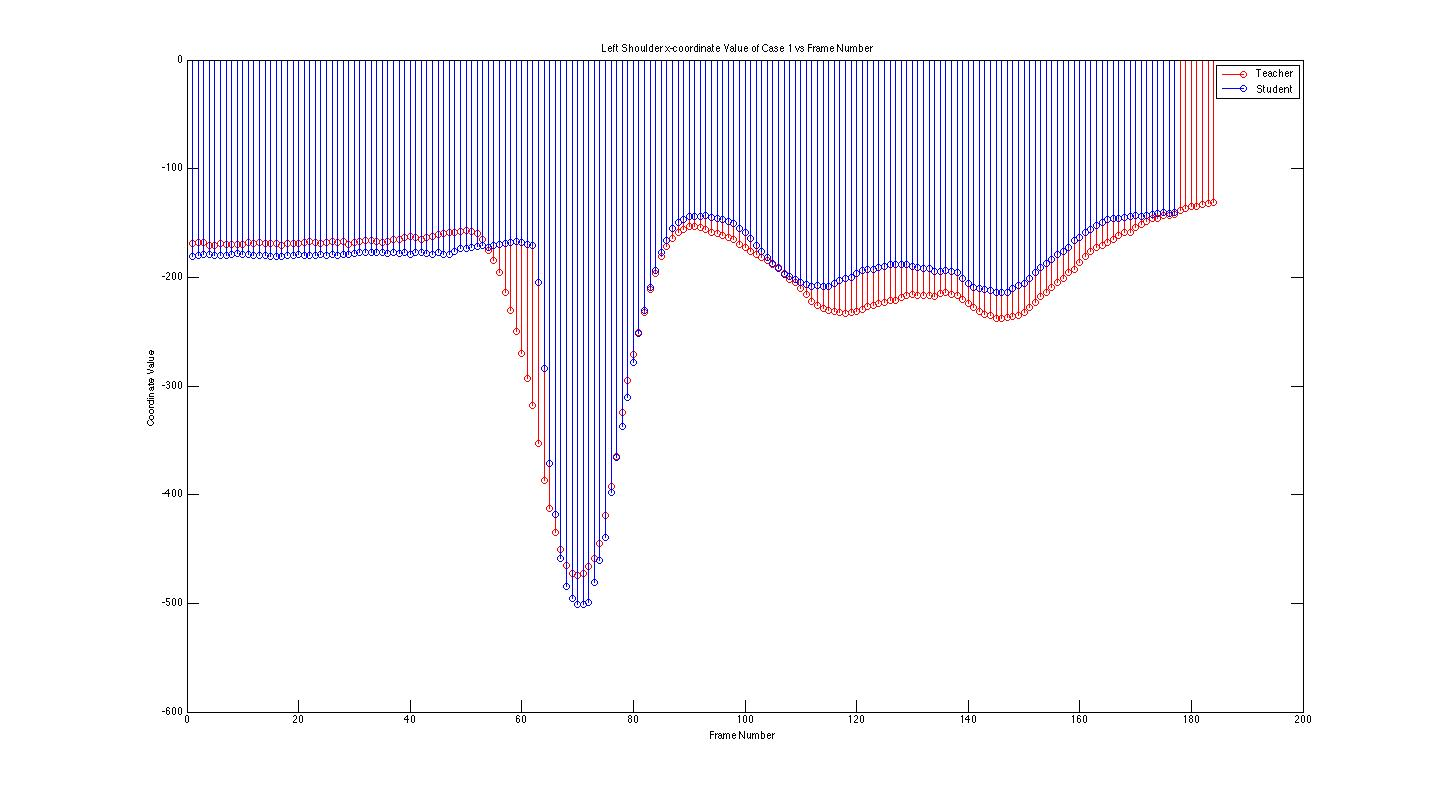
\includegraphics[scale=0.3]{Data_Analysis_LS_Correct.jpg}
\caption{Left Shoulder x-coordinate data of teacher and student. As it can be seen the student makes an error at roughly frame 50 and is also off from about frame 120 to 160.}
\label{error_left_shoulder}
\end{figure}

\subsubsection{Results}
\noindent
The graphs in Figure \ref{error_score} show the results of test cases 1 to 4. As it is clear, the more closely the student represents the dance, the lower the error (top left) and the higher the score (top right). This is both in the average score case, and in the time framed case. In Case 1, though the student tries to replicate the dance the same, it can clearly be seen in the windowed results that this is not the case and once the window is identified, the joint(s) which made the error can also be identified. In this case it appears to be the x-coordinate of the left shoulder as can be seen in Figure \ref{error_left_shoulder}. Whether or not this should be penalised so much since the overall movement is quite similar, is not discussed here as this is more of a subjective issue. It is also clear that in the Case 2 and Case 3 scenario only some of the windows are given a low score, whereas in the rest of them the error is comparable to that of Case 1. This follows the video data as the student makes two errors with the arms within the periods of time that are represented by the windows. Finally, Case 4 shows a low score for almost all of the window frames as predicted. 

\subsubsection{Score Function}
\noindent
These results show that there is a great need for user friendly feedback of the results. One thing to note is that firstly, the results are given in an unintuitive scale for the regular daily user. Added to this is the fact that the results are not bounded in any way. Ideally, we would like for a good score to get something that appears to be close to 100\% and a bad score to get close to 0\%. To do this, we may use a variation of the sigmoid function that has these properties.
\begin{equation}
S(\epsilon) = 100\left[\underbrace{\frac{1}{1+e^{\left(a\epsilon-b\right)}}}_{SigmoidFunction} + \underbrace{\left(1 - \frac{1}{1 + e^{-b}}\right)}_{Offset}\right]
\end{equation}

	where the $Offset$ is added so that the scoring function $S$ is bounded in the range [0,100].
\\\\
\noindent
By passing the estimated error $\epsilon$ through the modified sigmoid function $S$, we obtain a score in the range of $[0,100]$ which complies with most conventional scoring schemes and thus is more intuitive. Moreover, to retain a smooth transition along the range [20,80], we select the scaling and shifting factors, $a$ and $b$ respectively, in accordance to our tests' results. The final selected values are 10 and 3 for $a$ and $b$ respectively. The calibrated sigmoid function can be seen below in Figure \ref{score_function}.

\begin{figure}[H]
\centering
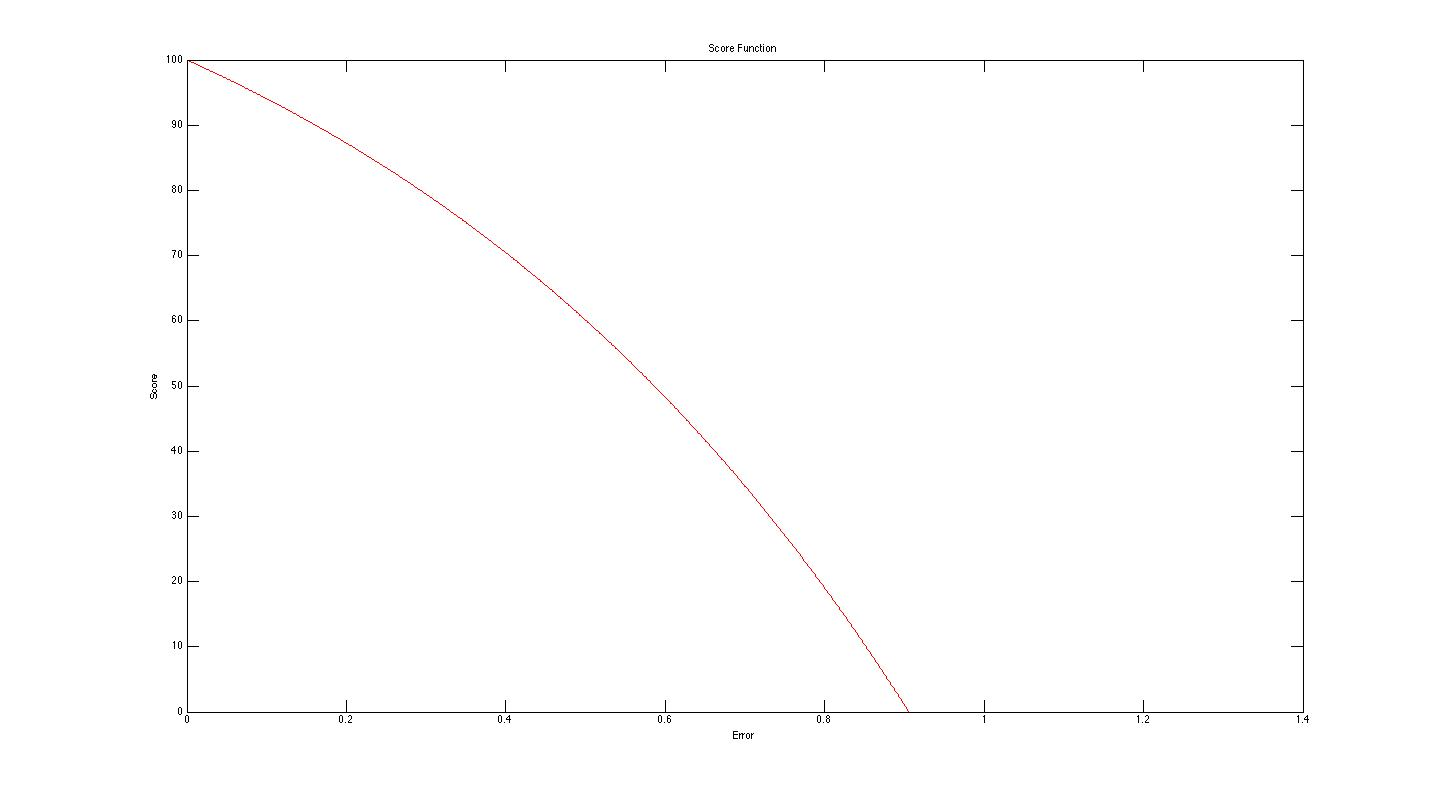
\includegraphics[scale=0.3]{Score_Function.jpg}
\caption{Graph of scoring function.}
\label{score_function}
\end{figure}
\noindent
The following figure (Figure \ref{error_score}) illustrates the transformation of an unbounded and unintuitive error estimate $\epsilon$ to a user friendly score. The top left figure shows the overall error of the four test cases while the top right one shows the actual calculated score for these errors. The detailed score per window for each test case can be seen in the four bottom graphs.

\begin{figure}[H]
\centering
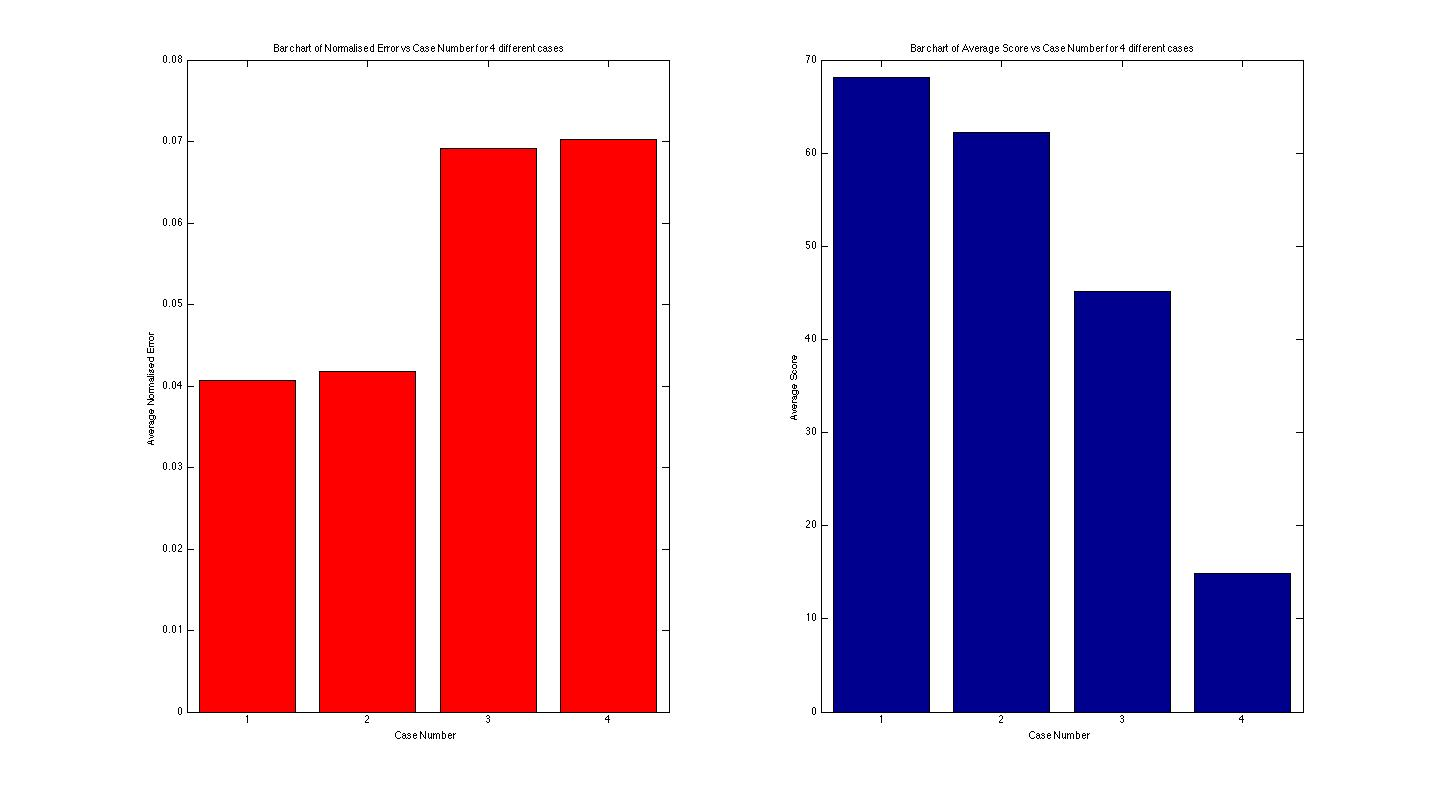
\includegraphics[scale=0.2]{Data_Analysis_Average_Score.jpg}
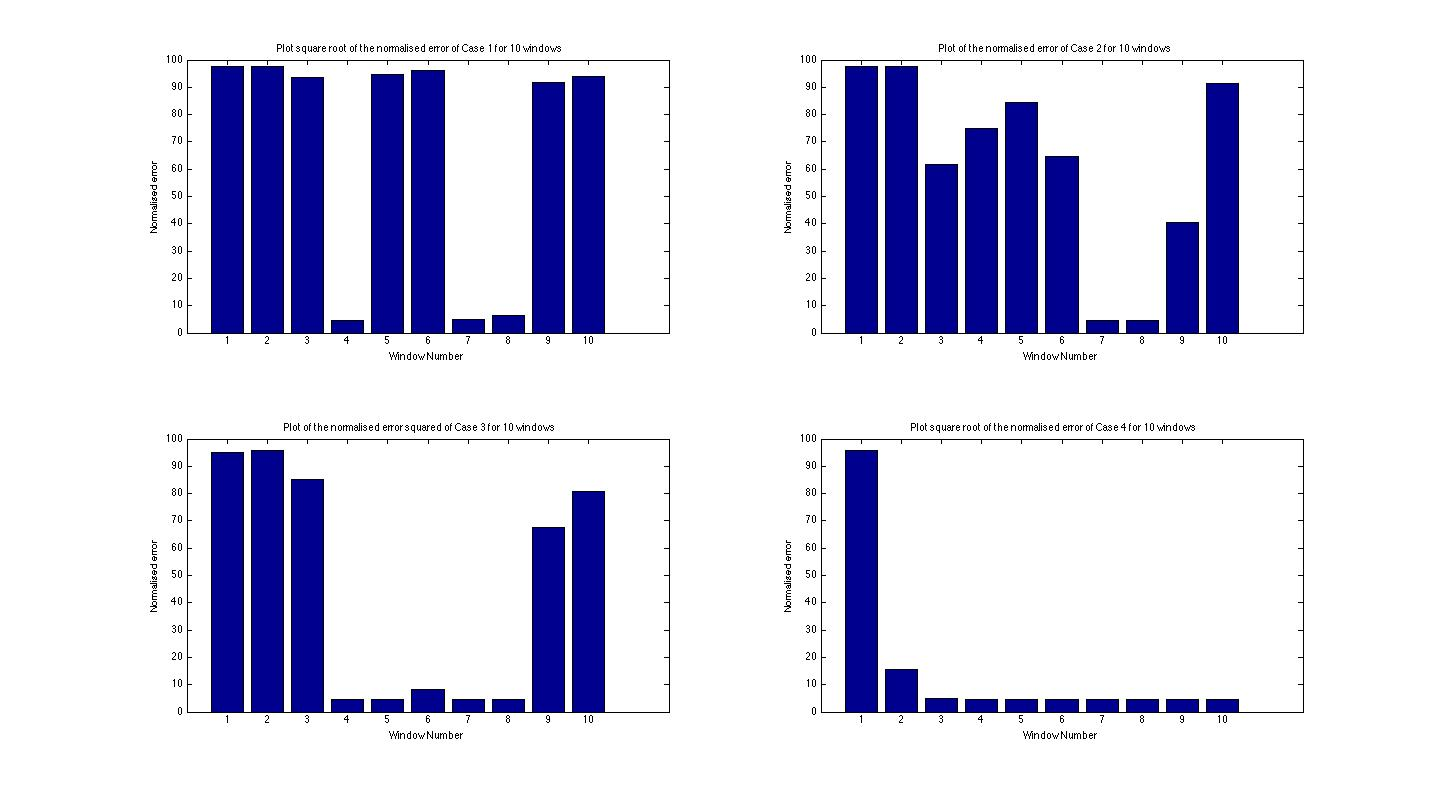
\includegraphics[scale=0.2]{Data_Analysis_Window_Score.jpg}

\caption{Overall error of the four test cases (top left) and score calculated for these errors (top right). Score calculated for four test cases split into 10 portions of time (bottom four graphs).}
\label{error_score}
\end{figure}

\clearpage
\section{Porting to C++}
\noindent
To make the code quicker and to make the whole application integrate more easily it has been chosen to port all the code, written initially in Matlab, to C++. 
\subsection{Linear Algeabra Library Choice}
This has been made much more time efficient by the use of the external library chosen for linear algeabra called Armadillo.  The reason this library has been chosen is due to its similarity in syntax to Matlab but also due to its speed. Armadillo claims on its website \textbf{(Add reference http://arma.sourceforge.net/speed.html)} to be approximately up to 15 times faster for the operations that are needed for our algorithms than two competing libraries IT++ and NEWMAT. Also being well established and well documented, the transition has been fairly simple.  
\subsection{Design}
\begin{itemize}
\item Abstraction.
\item Two Classes.
\item Public and Private.
\end{itemize}
\subsection{Development}
\noindent
\subsubsection{Unit Testing}
\noindent 
The code has been tested on a unit bases. Every method created in C++ has been tested against its Matlab counterpart. The development is as follows:
\begin{itemize}
\item For each method. 
\item Write small programme in C++ that calls method (before being created) and prints results in a text file in the Matlab DataFiles directory able to be loaded into Matlab.
\item Write the method in C++.
\item Write a script in Matlab that calls the corresponding Matlab function and then loads the text file created by the C++ program and compares the two results.
\end{itemize}
\noindent
This way the possibility of finding an error before it is buried deep within the code is minimised and the process of testing is automised. Added to this, the code can be easily divided between different pairs as the code can be decoupled. As long as the specification of each function is clear including what must be returned for each of the methods, each pair can easily test and debug their part of the code without the need to wait for previous code to be made.

\subsubsection{Integration}
\noindent
The final code is tested by making a test program that calls the analyse procedure in C++ and prints all the member variables to text files. This again is tested agains the Matlab results using a script in the same way as in the unit testing.   


\clearpage
\section*{Appendix}
\subsection*{Some Code}
\begin{lstlisting}
int main()
{
	// your code
	x = 5;
	// our code
}

\end{lstlisting}
\end{document}
